\documentclass[a4paper,12pt, oneside]{book}

% \usepackage{fullpage}
\usepackage[italian]{babel}
\usepackage[utf8]{inputenc}
\usepackage{amssymb}
\usepackage{amsthm}
\usepackage{graphics}
\usepackage{amsfonts}
\usepackage{listings}
\usepackage{amsmath}
\usepackage{amstext}
\usepackage{engrec}
\usepackage{rotating}
\usepackage{verbatim}
\usepackage[safe,extra]{tipa}
% \usepackage{showkeys}
\usepackage{multirow}
\usepackage{hyperref}
\usepackage{microtype}
\usepackage{fontspec}
\usepackage{enumerate}
\usepackage{physics}
\usepackage{braket}
\usepackage{marginnote}
\usepackage{pgfplots}
\usepackage{cancel}
\usepackage{polynom}
\usepackage{booktabs}
\usepackage{enumitem}
\usepackage{framed}
\usepackage{pdfpages}
\usepackage{pgfplots}
\usepackage{algorithm}
% \usepackage{algpseudocode}
\usepackage[cache=false]{minted}
\usepackage{mathtools}
\usepackage[noend]{algpseudocode}
\newcommand*{\bfrac}[2]{\genfrac{}{}{0pt}{}{#1}{#2}}

\usepackage{tikz}\usetikzlibrary{er}\tikzset{multi  attribute /.style={attribute
    ,double  distance =1.5pt}}\tikzset{derived  attribute /.style={attribute
    ,dashed}}\tikzset{total /.style={double  distance =1.5pt}}\tikzset{every
  entity /.style={draw=orange , fill=orange!20}}\tikzset{every  attribute
  /.style={draw=MediumPurple1, fill=MediumPurple1!20}}\tikzset{every
  relationship /.style={draw=Chartreuse2,
    fill=Chartreuse2!20}}\newcommand{\key}[1]{\underline{#1}}
\usetikzlibrary{arrows.meta}
\usetikzlibrary{decorations.markings}
\usetikzlibrary{arrows,shapes,backgrounds,petri}
\tikzset{
  place/.style={
    circle,
    thick,
    draw=black,
    minimum size=6mm,
  },
  transition/.style={
    rectangle,
    thick,
    fill=black,
    minimum width=8mm,
    inner ysep=2pt
  },
  transitionv/.style={
    rectangle,
    thick,
    fill=black,
    minimum height=8mm,
    inner xsep=2pt
  }
} 
\usetikzlibrary{automata,positioning,chains,fit,shapes}
\usepackage{fancyhdr}
\pagestyle{fancy}
\fancyhead[LE,RO]{\slshape \rightmark}
\fancyhead[LO,RE]{\slshape \leftmark}
\fancyfoot[C]{\thepage}
\usepackage[usenames,dvipsnames]{pstricks}
\usepackage{epsfig}
\usepackage{pst-grad} % For gradients
\usepackage{pst-plot} % For axes
\usepackage[space]{grffile} % For spaces in paths
\usepackage{etoolbox} % For spaces in paths
\makeatletter % For spaces in paths
\patchcmd\Gread@eps{\@inputcheck#1 }{\@inputcheck"#1"\relax}{}{}
\makeatother

\title{Fondamenti Logico Matematici dell'Informatica}
\author{UniShare\\\\Davide Cozzi\\\href{https://t.me/dlcgold}{@dlcgold}}
\date{}

\pgfplotsset{compat=1.13}
\begin{document}
\maketitle

\definecolor{shadecolor}{gray}{0.80}
\setlist{leftmargin = 2cm}
\newtheorem{teorema}{Teorema}
\newtheorem{definizione}{Definizione}
\newtheorem{esempio}{Esempio}
\newtheorem{corollario}{Corollario}
\newtheorem{lemma}{Lemma}
\newtheorem{osservazione}{Osservazione}
\newtheorem{nota}{Nota}
\newtheorem{esercizio}{Esercizio}
\algdef{SE}[DOWHILE]{Do}{doWhile}{\algorithmicdo}[1]{\algorithmicwhile\ #1}
\tableofcontents
\renewcommand{\chaptermark}[1]{%
  \markboth{\chaptername
    \ \thechapter.\ #1}{}}
\renewcommand{\sectionmark}[1]{\markright{\thesection.\ #1}}
\newcommand{\floor}[1]{\lfloor #1 \rfloor}
\newcommand{\MYhref}[3][blue]{\href{#2}{\color{#1}{#3}}}%
\chapter{Introduzione}
\textbf{Questi appunti sono presi a lezione. Per quanto sia stata fatta
  una revisione è altamente probabile (praticamente certo) che possano
  contenere errori, sia di stampa che di vero e proprio contenuto. Per
  eventuali proposte di correzione effettuare una pull request. Link: }
\url{https://github.com/dlcgold/Appunti}.\\
\chapter{Dimostrazioni = Algoritmi}
Parliamo in primis del \textbf{paradigma dimostrazioni = algoritmi}.\\
Prendiamo come \textit{linguaggio di specifica} un \textbf{linguaggio
  del prim'ordine con identità}.
\begin{shaded}
  Si riportano alcune definizioni utili in \textit{logica matematica} tratte da
  Wikipedia: 
  \begin{definizione}
    Definiamo \textbf{linguaggio del primo ordine} come un linguaggio formale
    che serve per gestire meccanicamente enunciati e ragionamenti che
    coinvolgono i connettivi logici, le relazioni e i quantificatori $\forall$ e
    $\exists$.\\
    Si ha che ``del primo ordine'' ndica che c'è un insieme di riferimento e i
    quantificatori possano riguardare solo gli elementi di tale insieme e non i
    sottoinsiemi (posso dire ``per tutti gli elementi'' ma non ``per tutti i
    sottoinsiemi''). Tale linguaggio è caratterizzato da:
    \begin{itemize}
      \item un \textbf{alfabeto di simboli} per variabili, costanti, predicati,
      funzioni, connettivi, quantificatori o punteggiatura 
      \item un \textbf{insieme di termini} per denotare gli elementi
      dell'insieme in analisi
      \item un \textbf{insieme di formule ben formate (\textit{FBF})} ovvero un
      insieme di stringhe composte di simboli dell'alfabeto che vengono
      considerate sintatticamente corrette 
    \end{itemize}
  \end{definizione}
  \begin{definizione}
    Definiamo \textbf{sistema assiomatico} come un insieme di assiomi che
    possono essere usati per dimostrare teoremi. Una teoria matematica consiste
    quindi in una assiomatica e tutti i teoremi che ne derivano.  
  \end{definizione}
  \begin{definizione}
    Definiamo un sistema formale come una formalizzazione rigorosa e completa
    della nozione di sistema assiomatico costituito da:
    \begin{itemize}
      \item un alfabeto
      \item una grammatica che specifica quali sequenze finite dei simboli
      dell'alfabeto corrispondono ad una FBF. La grammatica deve essere
      ricorsiva, nel senso che deve esistere un algoritmo per decidere se una
      sequenza di simboli è o meno una formula ben formata 
      \item un sottoinsieme delle FBF che sono gli assiomi. L'insieme degli
      assiomi è ricorsivo
      \item le regole di inferenze che associano formule ben formate ad n-uple
      di formule ben formate
    \end{itemize}
  \end{definizione}
  \begin{definizione}
    Definiamo gli \textbf{assiomi di Peano} come un gruppo di assiomi ideati al
    fine di definire assiomaticamente l'insieme dei numeri naturali:
    \begin{itemize}
      \item esiste un numero naturale: 0 (alternativamente 1 se si vuole escludere
      0):
      \[0/1\in \mathbb{N}\]
      \item ogni naturale ha un naturale come successore. Ho quindi una funzione
      ``successore'' tale che:
      \[S:\mathbb{N}\to\mathbb{N}\]
      \item numeri diversi hanno successori diversi, ovvero:
      \[x\neq y\to S(x)\neq S(y)\]
      \item 0 (o alternativamente 1) non è il successore di alcun naturale,
      ovvero:
      \[S(x)\neq 0, \forall x\in \mathbb{N}\]
      \item ogni sottoinsieme di numeri naturali che contenga lo zero e il
      successore di ogni proprio elemento coincide con l'intero insieme dei
      numeri 
      naturali. Ovvero dato $U\subseteq \mathbb{N}$ tale che:
      \begin{itemize}
        \item $0\in U$
        \item $x\in U\to S(x)\in U$
      \end{itemize}
      allora:
      \[U=\mathbb{N}\]
      Tale assioma è detto \textbf{assioma dell'induzione} o \textbf{principio di
        induzione} 
    \end{itemize}
  \end{definizione}
  \begin{definizione}
    In una teoria del primo ordine si chiama \textbf{chiusura universale} di una
    formula ben formata $A(x_1,\ldots,x_n)$, con $x_1,\ldots,x_n$ variabili
    libere, la formula:
    \[\forall x_1\forall x_2\forall x_n\,\,A(x_1,\ldots,x_n)\]
    ottenuta premettendo un quantificatore universale su ogni variabile libera. 
  \end{definizione}
  \begin{definizione}
    Definiamo, in logica matematica, \textbf{aritmetica di Peano (\textit{PA})}
    come una teoria del primo 
    ordine che ha come assiomi propri una versione degli \textbf{assiomi di
      Peano} 
    espressi nel linguaggio del primo ordine. Si ha quindi che il linguaggio di
    PA 
    è il linguaggio dell'aritmetica del primo ordine con i seguenti simboli:
    \begin{itemize}
      \item vari simboli per le variabili: $x$, $y$, $z$, $x_1$ etc$\ldots$
      \item costanti individuali: $0$ etc$\ldots$
      \item simboli per funzioni unarie: $S$
      \item simboli per funzioni binarie $+$, $\times$ ($+(x,y)$ si indica anche
      con $x+y$ e analogamente si fa per $\times$)
      \item simboli per relazioni unarie: $=$
      \item simboli per connettivi logici, quantificatori e parentesi
    \end{itemize}
    Gli assiomi di PA sono costituiti da:
    \begin{itemize}
      \item gli assiomi logici
      \item gli assiomi per l'uguaglianza
      \item i seguenti assiomi propri (che ``traducono'' nella logica di Peano
      gli assiomi di Peano):
      \begin{itemize}
        \item $\forall x\neg(S(x)=0)$
        \item $\forall x\forall y(S(x)=S(y)\to x=y)$
        \item $\forall x(x+0=x)$
        \item $\forall x\forall y(x+S(y)=S(x+y))$
        \item $\forall x(x\times 0 =0)$
        \item $\forall x\forall y(x\times S(y)=(x\times y)+x)$
      \end{itemize}
    \end{itemize}
    Agli assiomi propri si aggiunge anche il seguente assioma proprio:
    {\footnotesize{\[(\phi(0,x_1,\ldots,x_n)\land(\forall
      x(\phi(x,x_1,\ldots,x_n)\to\phi(S(x),x_1,\ldots,x_n))\to\forall 
      x\phi(x,x_1,\ldots,x_n)\]}}
    per ogni FBF $\phi(x,x_1,\ldots,x_n)$ di cui
    $x,x_1,\ldots,x_n$ sono variabili libere. Questo è uno schema di assiomi
    detto \textbf{schema di induzione} e si ha un assioma per ogni FBF
    $\phi$ 
  \end{definizione}
  \begin{definizione}
    Definiamo, in logica classica, il \textbf{principio del terzo escluso} che
    stabilisce che una proposizione e la sua negazione hanno valore opposto, non
    avendo una ``terza opzione''. In logica classica è una \textbf{tautologia}.
  \end{definizione}
  \begin{definizione}
    Un termine è un \textbf{termine chiuso} sse non contiene delle variabili
    individuali.  
  \end{definizione}
  \begin{definizione}
    Una \textbf{formula chiusa} è una formula costruita nel linguaggio dei
    predicati in cui o non compaiono variabili o tutte le variabili presenti
    sono vincolate a un quantificatore e sono dunque variabili legate. 
  \end{definizione}
\end{shaded}
\begin{esempio}
  Vediamo qualche esempio:
  \[\forall x,y\in\mathbb{N},\,\,\exists z\in\mathbb{N}\mbox{ t.c. }
    mcd(x,y,z)\]
  ovvero $z$ è l'\textit{mcd} di $x$ e $y$.\\
  Un altro esempio:
  \[\forall x\in \mathbb{N},\,\,\exists y\in \mathbb{N}\mbox{ t.c. }
    fatt(x,y)\]
  ovvero $y$ è il fattoriale di $z$.
\end{esempio}
Formule come quelle dell'esempio possono essere lette come \textbf{specifiche
  del problema di trovare un algoritmo totalmente corretto} che calcoli il
risultato di tale problema per ogni input valido. Questa lettura non è implicita
nella logica classica, dove non è richiesto di stabilire come viene prodotto il
risultato. Si ha quindi a che fare con una lettura di un problema algoritmico di
interesse per un informatico.\\
Le \textbf{dimostrazioni} di questa tipologia di formule, nell'ambito
dell'\textbf{aritmetica di Peano (\textit{PA})}, sono quindi interpretabili come
gli algoritmi che calcolano le funzioni specificate. \\
Come \textit{vantaggi} di questa ``atteggiamento'' si ha che:
\begin{itemize}
  \item l'attenzione si concentra su costruire la dimostrazione, sui passi
  dimostrativi, e non sulla stesura del codice
  \item i passi elementari della dimostrazione sono automatici
  \item la correttezza della dimostrazione è verificabile in modo automatico
  \item l'estrazione/sintesi dell'algoritmo dalla dimostrazione è diretta. Una
  volta che si ha la dimostrazione corretta si può estrarre direttamente
  l'algoritmo. Tale algoritmo è totalmente corretto rispetto alla specifica
\end{itemize}
La difficoltà si trasferisce dall'ambito convenzionale della programmazione e
codifica dell'algoritmo in se alla costruzione dimostrazione e dei passi
dimostrativi.\\
Si hanno quindi anche degli \textit{svantaggi}, abbastanza problematici:
\begin{itemize}
  \item l'algoritmo ottenuto non è ottimale rispetto al problema. Rispetto a
  questo bisognerebbe capire come incorporare ``più semantica'' del problema da
  risolvere nella dimostrazione stessa
  \item il formalismo e il linguaggio delle dimostrazioni sono ``lontani'' da
  quelli usati usualmente nella pratica informatica
\end{itemize}
\textbf{Non tutte le dimostrazioni sono direttamente interpretabili come
  algoritmi}. Per vedere questa cosa prendiamo un esempio famoso di formula da
dimostrare in analisi.
\begin{esempio}[esempio di Troelstra]
  Esistono due numeri irrazionali $n$ e $m$ tali che $n^m$ è razionale. In
  termini di formula del primo ordine si ha quindi:
  \[\exists n,m\in\{\mathbb{R}/\mathbb{Q}\}\mbox{ t.c. }n^m\in\mathbb{Q}\]
  Cerchiamo di capire se:
  \[\sqrt{2}^{\sqrt{2}}\in \mathbb{Q}\mbox{ o }\sqrt{2}^{\sqrt{2}}\not\in
    \mathbb{Q}\]
  Vediamo quindi i due casi (sono solo due per il principio del terzo escluso):
  \begin{enumerate}
    \item assumo $\sqrt{2}^{\sqrt{2}}\in \mathbb{Q}$ e pongo $n=m=\sqrt{2}$
    avendo trovato due numeri irrazionali $n$ e $m$ tali per cui
    $n^m\in\mathbb{Q}$ 
    \item assumo $\sqrt{2}^{\sqrt{2}}\not\in \mathbb{Q}$ e pongo
    $n=\sqrt{2}^{\sqrt{2}}$ e $m=\sqrt{2}$. Ne segue che:
    \[n^m=\left(\sqrt{2}^{\sqrt{2}}\right)^{\sqrt{2}}=(\sqrt{2})^2=2\in\mathbb{Q}\] 
    e quindi ho due numeri irrazionali $n$ e $m$ tali per cui $n^m\in\mathbb{Q}$
  \end{enumerate}
  Non possiamo essere soddisfatti di questa dimostrazione. Non veniamo a
  conoscenza, tramite la dimostrazione, che $\sqrt{2}^{\sqrt{2}}$ sia o meno
  razionale. Non possiamo capirlo in quanto assumo il terzo escluso e quindi non
  so quale dei due casi sia valido, non abbiamo un ``esiste'' costruttivo
  ($\exists n,m\in \{\mathbb{R}/\mathbb{Q}\}$) in quanto non sappiamo se
  $\sqrt{2}^{\sqrt{2}}$ è razionale o meno. Nonostante ciò al dimostrazione sta
  perfettamente ``in piedi'' ma non esibisce $n$ e $m$ in quanto non determina
  se $\sqrt{2}^{\sqrt{2}}\in\mathbb{Q}$.
\end{esempio}
Quanto successo nell'esempio di Troelstra non può succedere in un
\textbf{sistema costruttivo}.
\begin{definizione}
  Definiamo \textbf{sistema costruttivo} un sistema dove si hanno come
  \textit{requisiti minimali}: 
\begin{itemize}
  \item $S\vdash A\lor B\to S\vdash A\mbox{ oppure } S\vdash B$ quindi se
  nel sistema dimostro $A\lor B$ allora nel sistema dimostro $A$ o dimostro $B$,
  con $A$ e $B$ formule chiuse. Questa è la \textbf{disjunction property
    (\textit{DP})}  
  \item $S\vdash\exists xA(x)\to S\vdash A(t)$ quindi se ho dimostrato un
  esistenziale allora deve esistere un termine chiuso $t$ per cui dimostro
  $A(t)$ nel sistema. Questa è la \textbf{explicitly definibility property
    (\textit{EDP})}, detta anche \textbf{existence/witness property}
\end{itemize}
\end{definizione}
La logica classica quindi \textbf{non è un sistema costruttivo} perché in logica
classica riesco sempre a dimostrare $A\lor\neg A$ mentre nell'esempio di
Troelstra si nota come non si possa dimostrare né $A$ né $\neg A$. Quindi da una
dimostrazione classica di $A\lor\neg A$ io non tiro fuori una dimostrazione
classica di $A$ oppure una dimostrazione classica di $\neg A$ quindi non vale la
DP. Inoltre non vale nemmeno la EDP, ho dimostrato l'esistenza di $n$ e $m$ (che
sono termini chiusi) ma non ho trovato se vale la proprietà che siano
irrazionali. La logica classica quindi non è una logica costruttiva.
\section{Interpretazione BHK}
Passiamo quindi ad una semantica informale che per ogni costante logica associa
una condizione per la sua \textit{costruibilità}. Questa è
\textbf{l'interpretazione Brouwer-Heyting-Kreisel (\textit{BHK})}.
\begin{definizione}
  Presa una costruzione $\pi$ per questa semantica proposizionale si ha che:
  \begin{itemize}
    \item $\pi(A\land B)=\pi'(A)\mbox{ e } \pi''(B)$ ovvero una costruzione di
    $A\land B$ e uguale ad un'altra costruzione di $A$ \textbf{e} un'altra
    ancora di $B$ 
    \item $\pi(A\lor B)=\pi'(A)\mbox{ o } \pi''(B)$ ovvero una costruzione di
    $A\lor B$ e uguale ad un'altra costruzione di $A$ \textbf{o} un'altra ancora
    di $B$
    \item $\pi(A\to B)$ è una funzione  (o un funzionale, ovvero un
    insieme di funzioni) $f$ che associa ad ogni
    costruzione $\pi'(A)$ una costruzione $\pi''(B)$ tale che
    $\pi''=f(\pi')$. Quindi $f$ associa costruzioni di $A$ a costruzioni di $B$
    \item $\pi(\neg A)$ è una costruzione $\pi'$ di $A\to\bot$
  \end{itemize}
  Lato semantica predicativa si ha che, dato un dominio $D$ per la variabile
  $x$: 
  \begin{itemize}
    \item $\pi(\exists xA(x))=\langle c,\pi'\rangle|\,c\in D\mbox{ e
    }\pi'(A(c))$ quindi è uguale ad una coppia $=\langle c,\pi'\rangle$ tale che
    $c$ appartiene al dominio e $\pi'$ è una costruzione effettiva di $A(c)$
    \item $\pi(\forall xA(x))=$ è una funzione $f$ che associa ad ogni elemento
    $c\in D$ una costruzione $\pi'(A(c))$ tale che $\pi'=f(c)$
  \end{itemize}
\end{definizione}
Questa semantica ``naive'' ha alcune problematiche/aporie:
\begin{itemize}
  \item la BHK non specifica la costruzione di una formula atomica
  \item la BHK non dimostra il falso infatti nella costruzione di $\neg$
  associamo la costruzione del $\neg A$ a quella dell'implicazione, che è una
  costruzione che associa costruzioni di $A$ e costruzioni di $B$ e quindi
  nessuna costruzione potrebbe avere il falso (???)
\end{itemize}
Bisognerà quindi chiarire alcune restrizioni dell'interpretazione BHK.\\
Si hanno varie semantiche per il costruttivismo che hanno ``precisato'' la BHK:
\begin{itemize}
  \item la semantica della\textbf{realizzabilità ricorsiva} di Kleene
  \item la semantica dell'\textbf{interpretazione dialettica} di G\"{o}del
  \item la semantica delle \textbf{prove possibili} di Prawitz
  \item la semantica dei \textbf{problemi finiti} di Medvedev
\end{itemize}
Queste 4 semantiche sono coerenti con la BHK e quindi sono \textbf{semantiche
  del costruttivismo}.\\
Passiamo ora ad una definizione formale.
\begin{definizione}
  Definiamo come \textbf{sistema costruttivo} un sistema $S$:
  \[S=T+L\]
  dove:
  \begin{itemize}
    \item $T$ è una teoria con assiomi di forma particolare
    \item $L$ è una logica intuizionistica, che prendiamo come punto di partenza
    per il costruttivismo, con le sue estensioni
  \end{itemize}
  Non sempre comunque date $T$ e $L$ si ha che $S$ è un sistema costruttivo.
\end{definizione}
Un esempio di sistema costruttivo è dato dall'\textbf{aritmetica
  intuizionistica}, ovvero la PA interpretata all'interno della logica
intuizionistica. Altri esempi sono le \textbf{teorie con assiomi di Harrop},
teorie con assiomi $\forall\exists$ con matrice positiva priva di quantificatori
e con minimo modello di Herbrandt etc$\ldots$\\ 
Le clausole di Horn usate i Prolog hanno un
modello minimo di Herbrandt e hanno  assiomi $\forall\exists$ con matrice
positiva priva di quantificatori dove $\exists$ viene eliminato attraverso
skolemizzazione e il $\forall$ è implicito nelle regole del programma in quanto
tutte le $X$, $Y$ etc$\ldots$ si intendono quantificati universalmente.\\
Quindi la parte assiomatica di una teoria non basta a rendere costruttivo il
sistema anche se la logica è costruttiva. Tuttavia se si restringono le
assiomatizzazioni con formule del primo ordine di tipo particolare si possono
ottenere sistemi costruttivi in cui vale come minimo la \textit{DP} e la
\textit{EDP}.
\section{Deduzione naturale}
Vediamo un accenno della \textbf{deduzione naturale} ovvero di un
\textbf{calcolo diretto} (quindi differente dal calcolo indiretto dei
tableaux). Nella deduzione naturale si ha per ogni connettivo una \textbf{regola
di introduzione} $i$ e una \textbf{regola di eliminazione} $e$. Ad esempio se ho
$A$ e $B$ come premesse posso introdurre l'and con la regola d:i introduzione
dell'and: 
\[\frac{A\,\,\,\,B}{A\land B}i\land\]
Se invece ho $A\land B$ come premessa posso usare la regola di eliminazione
dell'and, producendo:
\[\frac{A\land B}{A}e\land\mbox{ oppure }\frac{A\land B}{B}e\land\]
Avendo quindi due regole di eliminazione per l'and.\\
Passiamo all'or. Ho due regole di introduzione:
\[\frac{A}{A\lor B}i\lor\mbox{ oppure }\frac{B}{A\lor B}i\lor\]
L'eliminazione della or è complessa e verrà trattata più avanti ma è della
forma:
\[\frac{A\lor B\,\,\,\,C\,\,\,\,C}{C}e\lor\]
Dove si ha che se se ho $A\lor B$ come premessa e assumendo $A$ ho $C$ ma anche
assumendo $B$ ho $C$ posso eliminare l'or e ottenere $C$.\\
Passiamo all'implicazione. Se ho come assunzione $A$ e da $B$ riesco a
dimostrare $B$ allora posso introdurre l'implicazione:
\[\frac{\stackrel{\stackrel{[A]}{\cdots}}{B}}{A\to B}i\to\]
Per l'eliminazione ho che, tramite \textbf{modus ponens}:
\[\frac{A\to B\,\,\,\,A}{B}e\to\]
Abbiamo poi la \textbf{regola del falso} che dice che dal falso segue qualsiasi
cosa: 
\[\frac{\bot}{B}\bot\]
e la regola dell'eliminazione della negazione che dice che se assumo $\neg A$ e
ottengo il falso significa che si è ottenuta una contraddizione e quindi elimino
il $\neg$:
\[\frac{\stackrel{[\neg A]}{\bot}}{A}e\neg\]
Passiamo al $\forall$. Se ho dedotto $A(p)$ per $p$ generico posso introdurre il
$\forall$:
\[\frac{A(p)}{\forall xA(x)}i\forall\]
Se ho come assunzione $\forall xA(x)$ posso dedurre un qualsiasi $A(t)$:
\[\frac{\forall xA(x)}{A(t)}e\forall\]
Possiamo fare l'equivalente per l'$\exists$, dove se esiste $A(t)$ posso dedurre
l'esistenza di un certo $x$ per cui vale $A(x)$:
\[\frac{A(t)}{\exists xA(x)}i\exists\]
L'eliminazione dell'esiste è complessa e verrà trattata più avanti ma è della
forma:
\[\frac{\exists xA(x)\,\,\,\,\stackrel{[A(p)]}{C}}{C}e\exists\]
Dove assumendo $\exists xA(x)$, assumendo $A(p)$ con $p$ generico e riuscendo ad
ottenere $C$ da quest'ultima assunzione con una serie di restrizioni posso
ottenere $C$ eliminando $\exists$.\\
Una dimostrazione in deduzione naturale è modulare alle logiche si vogliono
usare:
\begin{itemize}
  \item nelle dimostrazioni in logica classica utilizzo tutte le regole della
  deduzione naturale appena introdotte
  \item nelle dimostrazioni in logica intuizionistica non devo usare la regola
  di eliminazione della negazione
  \item  nelle dimostrazioni in logica minimale non devo usare la regola
  di eliminazione della negazione e nemmeno la regola che dal falso segue
  qualsiasi cosa
\end{itemize}
Possiamo quindi caratterizzare queste tre logiche e nelle ultime due, quella
intuizionistica e quella minimale, si può dimostrare che valgono DP e EDP mentre
non posso dire lo 
stesso per la logica classica. Si ha inoltre che:
\[\mbox{logica minimale}\subseteq\mbox{logica
    intuizionistica}\subseteq\mbox{logica classica}\]
Discorso diverso vale per le teorie, ovvero per i sistemi, dove
l'assiomatizzazione può fare la differenza portando anche fuori dalla
costruttività (se ad esempio assumo come assioma che $\forall xA(x)\lor\neg
A(x)$ e gli aggiungo la logica intuizionistica ottengo la logica classica che
non è costruttiva).\\
Una teoria specifica è l'aritmetica di Peano dove si hanno i seguenti assiomi:
\begin{itemize}
  \item $\forall x\neg(S(x)=0)$
  \item $\forall x\forall y(S(x)=S(y)\to x=y)$
  \item $\forall x(x+0=x)$
  \item $\forall x\forall y(x+S(y)=S(x+y))$
  \item $\forall x(x\times 0 =0)$
  \item $\forall x\forall y(x\times S(y)=(x\times y)+x)$
\end{itemize}
Dove si ha la regola d'identità che in realtà sono due, ovvero $id1$ e $id2$:
\[\frac{}{x=x}id1\mbox{ e } \frac{x=y\,\,\,\,A(x)}{A(y)}id2\]
Dove si ha anche il principio/regola d'induzione:
\[\frac{A(0)\,\,\,\,\stackrel{\stackrel{[A(j)]}{\cdots}}{A(S(j))}}{A(t)}ind\]
Dove se dimostro $A(0)$ e assunto $A(j)$ dimostro il successore di $A(j)$ allora
posso dedurre $A(t),\forall t$.
\begin{esempio}
  Vediamo ora un esempio con degli assiomi specifici, costruttivi:
  \begin{itemize}
    \item $pari(0)$
    \item $\forall x(pari(x)\to \neg pari(S(x)))$
    \item $\forall x(\neg pari(x)\to pari(S(x)))$
  \end{itemize}
  Quindi si ha che se $x$ è apri non lo è il successore e se $x$ non è pari lo è
  il successore. Assumiamo inoltre che 0 sia pari.\\
  \textup{Scritta così potrebbe essere riscritta ``1:1'' in Prolog.}\\
  Cerchiamo quindi din dimostrare che che:
  \[\forall x(pari(x)\lor \neg pari(x))\]
  che si può pensare si un terzo escluso e quindi valga sempre. Questa formula,
  a 
  livello di specifica, va letta come una funzione ``per ogni numero naturale
  costruisce $pari(x)$ o $\neg pari(x)$'' quindi costruisce o la parte sinistra
  o 
  la parte destra. Quindi la formula i può leggere come la specifica di
  algoritmo 
  che per ogni naturale mi dice se vale la parte sinistra o la parte destra
  dell'or e quindi è un algoritmo di decisione effettivo che per ogni naturale
  ti 
  dice se è pari o non è pari. Questa è un'interpretazione diversa da quella
  classica. \\
  Posso quindi fare una dimostrazione per induzione.\\
  Il \textbf{caso base} è, chiamando $pari$ $p$, assunto per assioma $p(0)$ e
  usando l'introduzione dell'or:
  \[\frac{p(0)}{p(0)\lor \neg p(0)}i\lor\]
  Passo al \textbf{caso passo}.\\
  Assumo per ipotesi induttiva $p(j)\lor \neg p(j)$ e assumiamo $\forall
  x(p(x)\lor \neg p(S(x)))$ che è un altro degli assiomi. Procedo eliminando il
  $\forall$:
  \[\frac{\forall x(p(x)\lor \neg p(S(x)))}{p(j),p(j)\to\neg
      p(S(j))}e\forall\]
  procedo quindi eliminando l'implicazione:
  \[\frac{p(j),p(j)\to\neg
      p(S(j))}{\neg p(S(j))}e\to\]
  e continuo inserendo l'or:
  \[\frac{\neg p(S(j))}{p(S(j))\lor\neg p(S(j))}i\lor\]
  Analogamente faccio per l'altro assioma $\forall x(\neg p(x)\lor p(S(x)))$:
  \[\frac{\forall x(\neg p(S(x) )\lor  p(S(x)))}{\neg p(j),\neg p(j)\to
      p(S(j))}e\forall\]
  \[\frac{\neg p(j),\neg p(j)\to
      p(S(j))}{p(S(j))}e\to\]
  \[\frac{p(S(j))}{p(S(j))\lor\neg p(S(j))}i\lor\]
  Partendo quindi da $p(j)\lor \neg p(j)$ posso fare l'eliminazione dell'or
  ottenendo il \textbf{caso passo}:
  \[\frac{p(j)\lor\neg p(j)}{p(S(j))\lor\neg p(S(j))}e\lor\]
  e quindi posso concludere il passo induttivo:
  \[\frac{p(0)\lor \neg p(0)\,\,\,\,p(S(j))\lor\neg p(S(j))}{\forall
      x(p(x)\lor \neg p(x))}ind\]
  concludendo al dimostrazione costruttiva.\\
  Posso quindi dire che, essendo 0 pari, 1 è dispari e quindi 2 è pari, 3
  dispari etc$\ldots$ in pratica è un ciclo che parte dal caso base e poi decide
  per qualsiasi numero naturale. Possiamo quindi estrarre un algoritmo iterativo
  (potrei anche estrarne uno ricorsivo) da questa dimostrazione. Tale algoritmo
  è visualizzabile nell'implementazione C nel listing \ref{lst:pari}.
\end{esempio}
\begin{listing}
  \inputminted{c}{``code/pari.c''}
  \label{lst:pari}
  \caption{Codice C dell'algoritmo di calcolo pari creato dalla dimostrazione}
\end{listing}
Come detto algoritmi così sintetizzati non sono algoritmi ottimali e l'esempio
del pari o dispari è evidente. Normalmente si avrebbe infatti:
\begin{listing}[H]
  \inputminted{c}{``code/pariopt.c''}
  \label{lst:pari2}
  \caption{Codice C dell'algoritmo di calcolo pari ottimale}
\end{listing}
E quindi si ha un limite nella costruzione dell'algoritmo anche se il primo
sappiamo essere corretto (avendo applicato la deduzione naturale e l'induzione,
ho la garanzia che in quella assiomatizzazione il programma sia totalmente
corretto) mentre di quest'ultimo dovremmo dimostrare la correttezza. Nel primo
programma la componente funzionale della dimostrazione è data dalle varie
funzioni che si richiamano. L'algoritmo per ogni istanza calcola se vale la
parte sinistra o destra della disgiunzione in modo uniforme. Le funzioni si
deducono automaticamente dalla prova costruttiva. Niente di tutto ciò è
asseribile sull'algoritmo ottimo.\\ 
Parlando invece di Prolog avrei una situazione diversa. In Prolog ogni
computazione è un'\textit{istanza di dimostrazione} che varia di caso in caso e
quindi non si ha una dimostrazione generale. Possiamo dire che un programma
Prolog non rappresenta l'algoritmo che risolve il problema specificato per ogni
dato di input. Si ha quindi un diverso modello di calcolo/computazione.
\chapter{Logica Intuizionistica}
\section{Logica Intuizionistica Proposizionale}
La \textbf{logica intuizionistica proposizionale} è il primo paradigma che
trattiamo di \textbf{logica costruttiva}, dove appunto valgono la \textbf{DP} e
la \textbf{EDP}, che sono i due requisiti minimali per dire che una logica è
costruttiva. L'intuizionismo proposizionale è il paradigma minimale di logica
costruttiva. 
\subsection{Sintassi}
Iniziamo a parlare dell'intuizionismo proposizionale e già a livello di
linguaggio si ha una differenza tra la logica classica e quella
intuizionistica.\\
Il linguaggio della logica proposizione intuizionistica comprende i seguenti
\textit{simboli}: 
\begin{itemize}
  \item variabili proposizionali $A$, $B$, $C$, etc$\ldots$
  \item connettivi $\land$, $\lor$, $\neg$ e $\to$. Il $\neg$ è l'unico
  connettivo unario mentre gli altri sono connettici binari
  \item simboli ausiliari come ``$($'' e ``$)$'' utili a stabilire precedenze
  tra connettivi 
\end{itemize}
Una formula ben formata intuizionistica è definita così:
\begin{enumerate}
  \item ogni variabile proposizionale appartiene alle FBF
  \item se $A$ e $B$ sono FBF allora:
  \begin{itemize}
    \item $\neg A$
    \item $A\lor B$
    \item $A\land B$
    \item $A\to B$
  \end{itemize}
  appartengono alle FBF
  \item nient'altro appartiene alle FBF
\end{enumerate}
E fin qui non si hanno differenze con la logica classica.\\
La differenza rispetto alla logica classica si riscontra nel fatto che i 4
connettivi intuizionistici sono tra loro \textbf{completamente indipendenti}. In
logica classica invece potrei anche solo usare $\neg$ e $\lor$ in quanto gli
altri due si possono ricavare da questi due (tramite leggi di De Morgan
etc$\ldots$). In logica classica $\neg$ e $\lor$ formano un insieme minimale di
operatori. In logica intuizionistica non ho nulla del genere, non posso ridurre
nessun connettivo ad un altro. D'altro canto anche Prolog riduceva pesantemente
il linguaggio, basandosi sulla logica classica e sulle clausole di Horn anche
se si può aprire una discussione in merito al fatto che comunque la riduzione
del linguaggio delle clausole di Horn in Prolog comunque garantisce
l'algoritmicità delle dimostrazioni e la loro costruttività. Le clausole di Horn
sono infatti una restrizione del linguaggio classico e non tutte le formule di
logica classifica sono esprimibili in termini di clausole di Horn e questa è la
motivazione per cui il Prolog di fatto computa.\\
La logica classica pura non è costruttiva in quanto dimostro $A\lor \neg A$
anche se non è detto che poi siamo in grado di dimostrare $A$ o di dimostrare
$\neg A$. Il principio del terzo escluso fa ``saltare'' la costruttività della
logica classica, ``saltando'' la proprietà della disgiunzione DP.\\
Da un punto di vista formale quindi la logica intuizionistica ha l'alfabeto
della logica classica, la definizione di FBF della logica classica ma non si
hanno le equivalenze classiche che permettevano la riduzione del numero di
connettivi.\\ 
Le precedenze sui connettivi sono le stesse di quella logica classica e la
modifica delle precedenze avviene con lo stesso uso delle parentesi della logica
classica. Si ricorda che $\neg$ ha la precedenza su $\land$ che ha precedenza su
$\lor$ che ha precedenza su $\to$.\\
Con il simbolo $\vdash$ indichiamo la \textbf{dimostrabilità}. Quindi la
scrittura $\vdash A$, con $A\in FBF$, indica che la formula $A$ è dimostrabile
nella logica intuizionistica (in teoria bisognerebbe specificare la logica
a pedice di $\vdash$ ma se omesso, salvo diversamente specificato, si parla di
logica intuizionistica).\\
Passiamo quindi a presentare un \textbf{sistema deduttivo} per dimostrare
formule nella logica intuizionistica.\\
Partiamo con un sistema deduttivo molto semplice.\\
L'apparato deduttivo maneggerà due tipi di formule, che indichiamo come
\textbf{formule segnate} dai simboli $T$ e $F$. Data una qualsiasi FBF $A$
allora $TA$ e $FA$ sono formule segnate con $T$ e $F$.\\
Definiamo per ogni connettivo \textbf{T-regole} e \textbf{F-regole}. Suppongo
che $S$ sia un arbitrario insieme di formule segnate, con $/$ che specifica che
la regola si divide in due parti, con $S_T$ specifico che tengo di $S$ solo le
formule segnate con $T$ (sto facendo una \textit{restrizione}):
\begin{table}[H]
  \Large
  \centering
  \begin{tabular}{c||c|c}
    connettivo& T-regola& F-regola\\
    \hline
    \hline
    $\land$ & $T\land=\frac{S,T(A\land B)}{S,TA,TB}$&
                        $F\land=\frac{S,F(A\land B)}{S,FA/S,FB}$\\
    \hline
    $\lor$ & $T\lor=\frac{S,T(A\lor B)}{S,TA/S,TB}$&
                        $F\lor=\frac{S,F(A\lor B)}{S,FA,FB}$\\
    \hline
    $\to$ & $T\to=\frac{S,T(A\to B)}{S,FA/S,TB}$&
                        $F\to=\frac{S,F(A\to B)}{S_T,TA,FB}$\\
    \hline
    $\neg$ & $T\neg=\frac{S,T(\neg A)}{S,FA}$&
                        $F\neg=\frac{S,F(\neg A)}{S_T,TA}$\\
    \hline
  \end{tabular}
\end{table}
Senza le due restrizioni di $S$ a $_T$ otterrei i tableaux della logica classica
proposizionale. Quindi passare al questo apparato deduttivo della logica
intuizionistica non è complesso.\\
Usando queste regole una \textbf{dimostrazione} è una sequenze di applicazione
di queste regole che comincia sempre con $FX$ dove $X$ è la formula che voglio
dimostrare e deve terminare con una configurazione, ovvero un insieme di
sotto-dimostrazioni, che contiene una coppia complementare, ovvero una formula
segnata $T$ e la stessa formula segnata $F$. La logica intuizionistica (come 
quella classica) è \textbf{decidibile} quindi con un numero finito di passi
riesco sempre a stabilire se una formula è dimostrabile o meno nella logica
intuizionistica. Questo accade in quanto la lunghezza della formula è sempre
finita, non si ha possibilità di generare formule infinite, e le regole vanno a
destrutturare le formule ottenendo sempre formule di complessità minore ad ogni
applicazione di regola e quindi prima o pi si arriva alle formule atomiche,
finendo il processo in quanto non hanno ovviamente regole di destrutturazione.\\
Nella logica intuizionistica, a differenza di quella classica,
non tutti gli ordini di applicazione delle regole portano ad
una tavola chiusa, ovvero ad una dimostrazione della formula, anche se la
formula è dimostrabile. Esistono strategia di soluzione che non vanno a buon
fine e questo è dovuto all'ordine dell'applicazione delle regole e alla
concorrenza tra l'applicazione di due regole. Le uniche regole che però hanno
questo problema sono le due con restrizione. Non tutti (a priori rispetto
all'ordine di applicazione delle regole) i tableaux quindi sono
chiusi, a differenza della logica classica. Mi basta un tableaux chiuso (se
ottengo più branch per una regola devono comunque chiudere tutti) per
dimostrare che una formula è dimostrabile mentre per dire che non lo è mi serve
che tutti i possibili tableaux non siano chiusi. Si ricorda che non è necessaria
una formula atomica con $F$ e $T$ per chiudere un tableaux ma una qualsiasi FBF
con $F$ e $T$.
\begin{esempio}
  Vediamo che il principio del terzo escluso nell'intuizionismo non è
  dimostrabile.\\
  Prendo:
  \[A\lor \neg A\]
  e chiediamoci se è dimostrabile nella logica intuizionistica.\\
  So che non lo è quindi mi aspetto di non trovare un tableaux chiuso, ovvero
  che termina con tutti i rami che contengono una formula segnata $T$ e la stessa
  segnata $F$. Tale formula può essere diversa ramo per ramo anche se non
  succederà in questo caso avendo solo $A$.\\
  Parto segnando $F$ la formula:
  \[F(A\lor \neg A)\]
  Applico la $F$ di $\lor$:
  \[\frac{F(A\lor \neg A)}{FA,F(\neg A)}\]
  Applico ora l'unica regola che posso applicare, essendo $A$ atomica, ovvero
  la $F$ di $\neg$ (con praticamente $S=FA$ e quindi $S_T=\emptyset$):
  \[\frac{FA,F(\neg A)}{TA}\]
  Questo tableaux non è un tableaux chiuso e quindi la formula non è
  dimostrabile nella logica intuizionistica, come volevasi dimostrare.
\end{esempio}
\begin{esempio}
  Vediamo un'altro esempio.\\
  Prendiamo la legge di De Morgan:
  \[\neg (A\lor B)\to (\neg A)\land (\neg B)\]
  Parto con la dimostrazione:
  \[F(\neg (A\lor B)\to (\neg A)\land (\neg B))\]
  Procedo con l'implicazione:
  \[\frac{F(\neg (A\lor B)\to (\neg A)\land (\neg B))}{T(\neg (A\lor B)),F((\neg
      A)\land (\neg B))}\]
  Qui entra il problema della strategia. In questa situazione potrei applicare
  il $T$ di $\neg$ o l'$F$ di $\land$. Nella mia testa, o nel prover, devo
  comunque ricordare che ad un certo punto avevo la scelta, in modo da poter
  fare backtracking qualora non si chiuda il tableaux. Si ricorda che questo non
  poteva avvenire in logica classica. Lo segnalo con un
  asterisco:
  \[*T(\neg (A\lor B)),F((\neg A)\land (\neg B))\]
  Procedo prima con il $T$ di $\neg$:
  \[\frac{T(\neg (A\lor B)),F((\neg A)\land (\neg B))}{F(A\lor B), F((\neg
      A)\land (\neg B))}\]
  Ma anche qui ho più scelte (l'$F$ di $\lor$ e l'$F$ di $\land$), me lo segno
  con due asterischi: 
  \[**F(A\lor B), F((\neg A)\land (\neg B))\]
  Scelgo la $F$ di $\lor$ perché non crea branch:
  \[\frac{F(A\lor B), F((\neg A)\land (\neg B))}{FA, FB, F((\neg A)\land (\neg
      B))}\]
  Procedo con la $F$ di $\land$, creando due branch:
  \[\frac{FA, FB, F((\neg A)\land (\neg B))}{FA, FB, F(\neg A)/ FA, FB, F(\neg
      B)}\]
  Ma:
  \[\frac{FA, FB, F(\neg A)/ FA, FB, F(\neg B)}{TA/TB}\]
  e quindi il tableaux non è chiuso. Effettuo il backtracking cominciando dal
  primo asterisco. Torno alla formula e rimuovo l'asterisco:
  \[T(\neg (A\lor B)),F((\neg A)\land (\neg B))\]
  Applico quindi la $F$ di $\land$:
  \[\frac{T(\neg (A\lor B)),F((\neg A)\land (\neg B))}{T(\neg (A\lor B)),F(\neg
      A)/T(\neg (A\lor B)),F(\neg B)}\]
  Studiamo i due branch in parallelo ma devo mettere un asterisco, potendo fare
  sia $T$ che $F$ di $\neg$:
  \[*T(\neg (A\lor B)),F(\neg A)/T(\neg (A\lor B)),F(\neg B)\]
  Conviene fare il $F$ di $\neg$ perché conserviamo l'altra parte di formula:
  \[\frac{T(\neg (A\lor B)),F(\neg A)/T(\neg (A\lor B)),F(\neg B)}{T(\neg (A\lor
      B)),TA/T(\neg (A\lor B)),TB}\] 
  Procedo con la $T$ di $\neg$:
  \[\frac{T(\neg (A\lor B)),TA/T(\neg (A\lor B)),TB}{F(A\lor B),TA/F(A\lor B),
      TB}\]
  e quindi, con l'$F$ di $\lor$:
  \[\frac{F(A\lor B),TA/F(A\lor B), TB}{FA,FB,TA/FA,FB,TB}\]
  Nel primo branch ho $FA$ e $TA$ e quindi ho una formula con sia $F$ che $T$,
  ovvero $A$. Discorso analogo nel secondo con $B$ e quindi il tableaux è
  chiuso. Quindi questa legge di De Morgan è dimostrabile in logica
  proposizione intuizionistica. Mi basta una percorso che porta ad un
  tableaux chiuso (e volendo qui si potrebbe vedere che è anche l'unica facendo
  gli altri percorsi mancanti). \\
  Si può vedere, facendo i conti che l'altra formula di De Morgan:
  \[\neg (A\land B)\to (\neg A)\lor (\neg B)\]
  non è dimostrabile, non arrivando mai ad un tableaux chiuso. Non ho mai una
  strategia vincente  quindi la formula non è dimostrabile nella logica
  intuizionistica. Dietro a questo comportamento si ha un motivo semantico che
  vedremo.  
\end{esempio}
\begin{esempio}
  Tramite i tableaux si vede che la legge della doppia negazione:
  \[\neg\neg A\to A\]
  non è dimostrabile (per di più avendo un solo cammino) in logica
  intuizionistica. 
\end{esempio}
Si vedrà che la legge del terzo escluso o la legge della negazione, se aggiunti
(ne basta uno dei due)
alla logica intuizionistica la trasformano nella logica classica e viceversa, se
nella logica classica non dimostro il terzo escluso o la doppia negazione
ottengo la logica intuizionistica.
\begin{esempio}
  Tramite i tableaux si vede che la legge della conversa (non sono sicuro di
  aver sentito bene il nome):
  \[A\to \neg\neg A\]
  è dimostrabile (per di più avendo un solo cammino) in logica
  intuizionistica. \\ 
  Si può quindi vedere come valendo un solo verso dell'implicazione (non vale la
  legge della doppia negazione) non può valere l'equivalenza $A\iff\neg \neg A$
  in logica intuizionistica.
\end{esempio}
Il backtracking ha conseguenze nella complessità dell'algoritmo di decisione
della logica proposizionale intuizionistica che è stato dimostrato da Stackman
avere complessità spaziale pari a: 
\[O(n+\log n)\]
Il backtracking si può iterare a seconda dell'ordine delle regole.\\
Non posso dire nell'intuizionismo che vale $A$ sse non vale $\neg\neg
A$. Infatti il sse altro non è che:
\[A\iff\neg \neg A\]
e quindi dovrei avere sia che:
\[A\to\neg \neg A\]
\[\neg \neg A\to A\]
ma abbiamo solo la prima valida.
\begin{esempio}
  Ci chiediamo se la formula:
  \[A\to B\]
  equivale, come in logica classica, a:
  \[\neg A\lor B\]
  ovvero:
  \[A\to B\iff \neg A\lor B\]
  Già da subito possiamo dire che non vale in quanto si avrebbe dipendenza tra
  connettivi, cosa che abbiamo detto non esistere in logica intuizionistica.\\
  Vediamo se sono dimostrabili i due versi:
  \[(A\to B)\to(\neg A\lor B)\]
  \[(\neg A\lor B)\to(A\to B)\]
  Facendo i passaggi si dimostra che la prima formula non è dimostrabile e
  quindi già sappiamo che non vale il sse. Comunque possiamo fare i conti e
  veder che il secondo verso è dimostrabile in logica intuizionistica.
\end{esempio}
\noindent
Vediamo un trucco per le strategia:
\textit{se si ha una formula la cui regola restringe $S$ a $S_T$ se ho formule
complesse segnate $T$ mi conviene aspettare ad applicare queste $T$ e
applicare la $F$ delle regole che restringono, ovvero quelle di $\neg$ e
$\to$.}\\
Abbiamo quindi descritto un genuino sistema di decisione con però un piccolo
problema per il quale serve un esempio. 
\begin{esempio}
  Proviamo a vedere se la formula della doppia negazione del principio del terzo
  escluso è dimostrabile nella logica intuizionistica. Studiamo quindi la
  formula: 
  \[\neg\neg(A\lor \neg A)\]
  Si ha quindi:
  \[F(\neg\neg(A\lor \neg A))\]
  E quindi:
  \[\frac{F(\neg\neg(A\lor \neg A))}{T(\neg (A\lor \neg A))}\]
  Da cui segue:
  \[\frac{T(\neg (A\lor \neg A))}{F(A\lor \neg A)}\]
  Proseguendo:
  \[\frac{F(A\lor \neg A)}{FA, F(\neg A)}\]
  E infine:
  \[\frac{FA, F(\neg A)}{TA}\]
  Coi soliti passaggi si arriverebbe (si noti il condizionale) a dire che non è
  dimostrabile arrivando nell'unico percorso possibile ad un tableaux non
  chiuso. \\
  Anche Fitting arriva a questa conclusione
\end{esempio}
Ma per capire meglio il problema serve un teorema.
\begin{teorema}[Teorema di Kolmogorov-Glivenko]
  Se una formula $A$ è dimostrabile in logica classica allora e solo allora è
  dimostrabile in logica intuizionistica la doppia negazione di tale formula, a
  livello proposizionale (a livello predicativo se cose si complicano
  particolarmente). 
\end{teorema}
Ma questo stona rispetto all'esempio appena fatto. Il terzo escluso è
dimostrabile in logica classica e quindi ci aspetteremmo che la sua doppia
negazione sia dimostrabile in logica intuizionistica, contraddicendo il teorema.
Proviamo a rivedere i conti:
\[F(\neg\neg(A\lor \neg A))\]
E quindi:
\[\frac{F(\neg\neg(A\lor \neg A))}{T(\neg (A\lor \neg A))}\]
da cui segue:
\[\frac{T(\neg (A\lor \neg A))}{F(A\lor \neg A)}\]
applicando però $T$ di $\neg$ mi premuro di riscrivere la formula a cui ho
applicato la regola, ottenendo al posto del risultato precedente:
\[\frac{T(\neg (A\lor \neg A))}{F(A\lor \neg A), T(\neg (A\lor \neg A))}\]
questo complica molto il calcolo ma si dimostrerà che comunque ripetere le
formule non rende il calcolo infinito.\\
Ora avrei più scelte quindi lo segnalo con il solito asterisco:
\[*F(A\lor \neg A), T(\neg (A\lor \neg A))\]
Proseguo in primis con l'$F$ dell'or:
\[\frac{F(A\lor \neg A), T(\neg (A\lor \neg A))}{FA, F(\neg A), T(\neg (A\lor
    \neg A))}\]
Anche qui ho più scelte, lo segnalo:
\[**FA, F(\neg A), T(\neg (A\lor\neg A))\]
Proseguo con $F$ di $\neg$:
\[\frac{FA, F(\neg A), T(\neg (A\lor\neg A))}{TA, T(\neg (A\lor\neg A))}\]
Proseguo con $T$ di $\neg$:
\[\frac{TA, T(\neg (A\lor\neg A))}{TA, F(A\lor\neg A)}\]
E quindi:
\[\frac{TA, F(A\lor\neg A)}{TA, FA, F(\neg A)}\]
Avendo $TA$ e $FA$ mi posso fermare avendo chiuso il tableaux (si nota che
risolvere il $\neg$ avrebbe portato ad avere $TA,TA$ non chiudendo il
tableaux). Si è quindi dimostrato che la formula è dimostrabile, confermando
quanto detto nel teorema di di Kolmogorov-Glivenko.\\
Ripetere ogni volta la regola come fatto al secondo passaggio, però renderebbe
il tableaux ingestibile e renderebbe il calcolo semi-decidibile, perché se la
formula non è dimostrabile posso andare avanti all'infinito a ripetere le
formule, comportando un serio problema. Si nota inoltre che abbiamo subito
scelto il percorso che portava alla chiusura ma ci sono stati due punti in cui
abbiamo scelto una regola rispetto ad un'altra. La seconda scelta nella formula
con $*$ avrebbe portato ad un tableaux non chiuso (e si vedeva quasi ad occhio
che lo avrebbe fatto). Anche in merito alla formula con $**$ si nota che la
seconda scelta avrebbe portato ad un tableaux che non chiudeva. \\
Possiamo dire che la regola di poter riusare le formule a cui applichi la regola
riportandola nel tableaux è una sorta di \textbf{meta-regola}. L'aggiunta di
questa meta-regola è un calcolo completo rispetto alla logica proposizionale
intuizionistica, ovvero tutte le formule intuizionistiche dimostrabili hanno un
tableaux chiuso.\\
Le uniche formule che eventualmente richiedono al ripetizione, ovvero l'uso di
questa meta-regola, sono le formule $T$ di $\neg$ e $T$ di $\to$. Possiamo
quindi riformulare quelle due regole.\\
Per il $\to$:
\[T\to=\frac{S,T(A\to B)}{S,FA,T(A\to B)/S,TB}\]
notando che nella seconda parte non devo ripetere la formula.\\
Per il $\neg$:
\[T\neg=\frac{S,T(\neg A)}{S,FA,T(\neg A)}\]
Con le regole così modificate (queste due modificate più tutte le altre non
modificate) abbiamo un \textbf{calcolo completo e corretto} per la 
logica proposizionale intuizionistica. Non ci sono quindi formule dimostrabili
intuizionisticamente per cui non esiste un tableaux chiuso con le regole
descritte. D'ora in poi per i due casi useremo sempre le due nuove regole
modificate anche se potenzialmente non è sempre necessario. Se ottengo un
tableaux chiuso senza ripetizione lo ottengo anche con ma se lo ottengo con la
ripetizione non per forza lo ottengo senza. Volendo posso ricordarmi della
ripetizione usando un ``placeholder'' senza dover riscrivere ogni volta la
formula intera  per segnalare che in caso non riesca a
chiudere il tableaux senza la ripetizione posso usare la ripetizione.\\ 
Esplicitare i due casi in cui può servire la ripetizione della formula è un
grande aiuto dal punto di vista computazionale, essendo solo due casi.\\
\textit{In logica classica predicativa si ha una situazione analoga per quanto
  riguarda l'istanziazione dei parametri, con la $T$ di $\forall$ e la $F$ di
  $\exists$ (controllare appunti di fondamenti dell'informatica)}.\\
La logica classica proposizionale non richiederebbe mai un artificio simile a
quello della meta-regola, così come non richiede backtracking perché vale la
\textbf{proprietà di Chruch-Rosser} che ci assicura che se un tableaux deve
chiudere chiuderà qualsiasi percorso si scelga.\\
Ricordando che $\neg\neg A\to A$ non è dimostrabile intuizionisticamente ma
sappiamo che vale classicamente essendo una tautologia classica. Ma allora, per
il teorema di Kolmogorov-Glivenko al formula:
\[\neg\neg(\neg\neg A\to A)\]
è dimostrabile in logica intuizionistica e si può verificare coi soliti
passaggi (usando per di più una sola volta una ripetizione, nonostante
potenzialmente se ne creino di più durante la dimostrazione).
\subsection{Semantica e Modelli di Kripke}
Abbiamo parlato finora di \textbf{sintassi}, parliamo ora della
\textbf{semantica}, in termini di \textbf{modelli di Kripke}, per capire cosa
significano \textit{vero ($\top$)} e \textit{falso ($\bot$)} in logica
intuizionistica. La nozione di verità in logica intuizionistica è molto diversa
da quella della logica classica, dove ogni proposizione è semplicemente vera o
falsa sulla base delle tabelle di verità dei vari connettivi. La logica
intuizionistica non ha tale semantica perché assegna significati ai connettivi
in modo diverso dalla logica classica ma si basa appunto sui \textit{modelli di
  Kripke}. Kripke, prima dei modelli per l'intuizionismo, aveva chiuso un
problema per i modelli delle \textbf{logiche modali}, logiche dove si hanno gli
operatori di ``necessario'' e ``possibile'' associati alle formule che erano
divise in 5 logiche, S1, S2, S3, S4 e S5, ciascuna con semantiche diverse, anche
dal punto di vista del formalismo (non avendo una semantica che uniformasse
queste 5). Kripke, da giovane, ottenne una semantica unificatrice di queste 5
logiche modali, risolvendo questo problema aperto. Dopo la risoluzione di questo
problema Kripke si è appunto dedicato alla logica intuizionistica anche se i
suoi studi in merito (\textit{paper disponibile su Elearning}) hanno avuto
un'accoglienza ``tiepida'' in quanto si era in piena Guerra Fredda e gli studi
sul costruttivismo e sull'intuizionismo erano prevalentemente bandiera dell'est,
con Kolmogorov etc$\ldots$, mentre Kripke era statunitense, e quindi la Russia
contrastava tali studi se svolti da studiosi non dell'est (pubblicando solo in
russo per di più con una rivista negli USA che traduceva, in modo però non
integrale facendo riassunti, tali articoli). Un'altra accusa era
stata in merito al fatto che Kripke usava strumenti di logica classica per
parlare della semantica della logica intuizionistica. Alla fine erano due
motivazioni ideologiche e non tecniche.
\subsubsection{Modelli di Kripke in Intuizionismo Proposizionale}
\begin{definizione}
  Definiamo \textbf{modello di Kripke} per la logica intuizionistica
  proposizionale è una tripla:
  \[K=(G, R, \vDash)\]
  dove:
  \begin{itemize}
    \item $G$ insieme, finito o infinito, che Kripke chiama \textbf{stati di
      conoscenza}. Lo possiamo considerare come un \textbf{insieme discreto} di
    stati di conoscenza 
    \item $R$ relazione riflessiva e transitiva definita su $G$
    \item $\vDash$ ovvero una relazione tra elementi di $G$ e formule ben
    formate della logica intuizionistica. Tale relazione è detta
    \textbf{forcing} ovvero ``essere vero intuizionisticamente''.\\
    Formalmente diciamo che, dato $\Gamma\in G$ e $A\in FBF$ (nella logica
    intuizionistica), ``$\,\,\Gamma$ verifica $A$'' si scrive: $\Gamma\vDash
    A$. Quindi nello stato di conoscenza $\Gamma$ di tutti gli stati di
    conoscenza $G$ la formula $A$ è \emph{vera}. Se dico che, fissato $\Delta\in
    G$, $A$ è \emph{falsa} in $\Delta$ allora scrivo $\Delta\nvDash A$, avendo
    che ``$\,\,\Delta$ non verifica $A$'', quindi $A$ non è vera in $\Delta$
  \end{itemize}
\end{definizione}
Dobbiamo quindi caratterizzare la logica intuizionistica su questo modello. Si
richiede che se $\Gamma\in G$ rende vera $A\in FBF$ e $\Delta\in G$ è tale che
$\Gamma$ è in relazione $R$ con $\Delta$ allora anche $\Delta$ deve verificare
$A$, ovvero, formalmente:
\[\Gamma\vDash A \land \Gamma R\Delta\implies \Delta R A\]
Questo vale $\forall \Delta$ tale che $\Gamma R \Delta$.
Possiamo leggere quanto scritto anche nel seguente modo: \textit{una formula,
  quando è vera in uno stato di conoscenza $\Gamma\in G$ deve essere vera in
  tutti gli stati di conoscenza $\Delta\in G$ che si possono raggiungere da
  $\Gamma$}, questo perché la relazione $R$ è di tipo riflessivo e
transitivo. Tali stati vengono detti \textbf{stati compatibili}, in questo caso
con $\Gamma$. $\Gamma R \Delta$ si legge con ``$\Gamma$ è in relazione con
$\Delta$'' o anche  ``$\Delta$ è accessibile da $\Gamma$'' (soprattutto in
logica modale è detta \textbf{relazione di accessibilità}).\\
Una volta che una formula è vera in uno stato di conoscenza rimarrà
vero in tutti gli stati di conoscenza che seguono. Questo è un \textbf{requisito
  molto forte}, una volta che una formula diventa vera diventa vera per sempre,
in tutti i branch dell'albero a partire dal nodo in cui diventa vera. È quindi
vera in tutti gli stati di conoscenza compatibili a quello in cui diventa
vera. Se una formula è vera nella radice dell'albero rimarrà sempre vera, visto
che, avendo praticamente a che fare con un particolare \textbf{diagramma di
  Hasse}, dalla radice ``vedo'' tutti gli altri nodi.\\
La critica che viene fatta a questa teoria è che non si prevede la
\textbf{falsificabilità} di una formula. \\
Dobbiamo quindi definire cosa significhino (e l'ordine non è causale in quanto
le prime due ricalcano molto la definizione classica), con $\Gamma\in G$ e
$A,B\in FBF$: 
\begin{itemize}
  \item $\Gamma\vDash (A\lor B)$ (si noti che le parentesi sono per sola
  facilità di lettura, avrei potuto scrivere $\Gamma\vDash A\lor B$). 
  \item $\Gamma\vDash (A\land B)$ (si noti che le parentesi sono per sola
  facilità di lettura, avrei potuto scrivere $\Gamma\vDash A\land B$)
  \item $\Gamma\vDash \neg A$ 
  \item $\Gamma\vDash (A\to B)$ (si noti che le parentesi sono per sola
  facilità di lettura, avrei potuto scrivere $\Gamma\vDash A\to B$)
\end{itemize}
Si ha quindi che, con $\Gamma\in G$ e $A,B\in FBF$:
\begin{itemize}
  \item $\Gamma\vDash (A\lor B)$ sse $\Gamma\vDash A$ \textbf{o} $\Gamma\vDash
  B$  
  \item $\Gamma\vDash (A\land B)$ sse $\Gamma\vDash A$ \textbf{e} $\Gamma\vDash
  B$  
  \item $\Gamma\vDash \neg A$ sse $\Delta\nvDash A,\,\,\,\forall \Delta\in G
  \mbox{ t.c. } \Gamma R\Delta$. Si nota che è necessario anche che
  $\Gamma\nvDash A$ in quanto la relazione $R$ è riflessiva e quindi $\Gamma R
  \Gamma$ 
  \item $\Gamma\vDash (A\to B)$  sse \textbf{o} $\Delta\nvDash A$ \textbf{o}
  $\Delta\vDash B$,$\forall \Delta\in G \mbox{ t.c. } \Gamma R\Delta$. La
  definizione non mi dice che in tutti i $\Delta$ è falso $A$ o in tutti i
  $\Delta$ è vero $B$ ma può capitare che in alcuni sia falso $A$, in alcuni
  vero $B$. Mi basta che, per essere vera l'implicazione, in ogni $\Delta$ deve
  essere o falsa $A$ o vera $B$
\end{itemize}
Si nota che per i primi due non si ha una grande differenza rispetto alla logica
classica. Posso prendere un modello di Kripke in cui $G$ contiene un solo
elemento, che chiamiamo $\Gamma$, e ottenere la logica classica, che è quindi
caratterizzata da modelli di Kripke con un solo stato di conoscenza. Quindi
$\land$ e $\lor$ che si riferiscono allo stesso stato di conoscenza $\Gamma$
sono simili alla definizione classica di vero per $\land$ e $\lor$. Si vede che
per negazione e implicazione non vale un discorso simile, in quanto non si
prende più un solo stato di conoscenza tutti gli stati di conoscenza che sono in
relazione con $\Gamma$. Questa è una delle \textbf{caratterizzazioni} forti di
un connettivo nella logica intuizionistica.\\
Un'altra critica volta a Kripke è stata che, fissato un qualsiasi elemento di
$G$ in esso una formula o è vera o falsa \textit{classicamente}, e è stato
accusato di aver fatto una teoria dei modelli per una logica costruttiva, ovvero
l'intuizionismo, su base classica (cosa inaccettabile per gli intuizionisti
ortodossi). 
\textbf{Abbiamo dato la semantica della logica intuizionistica}.\\
Vediamo ora vari esempi di formule non dimostrabili intuizionisticamente, che
quindi non hanno un tableaux chiuso intuizionista, e per le quali deve quindi
esistere un \textbf{contromodello}, ovvero un modello di Kripke che falsifica
tali formule.
\begin{esempio}
  Cominciamo dalla non dimostrabilità del terzo escluso:
  \[\nvdash A\lor \neg A\]
  Dobbiamo mostrare un modello di Kripke che rende falsa questa formula.\\
  Disegno il modello di Kripke:
  \begin{figure}[H]
    \centering
    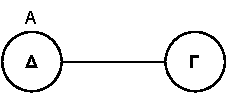
\includegraphics[scale = 0.9]{img/k1.pdf}
  \end{figure}
  Dove si hanno due nodi, $\Gamma$ e $\Delta$, e in cui se una FBF non viene
  indicata per un nodo significa che è falsa, mentre se viene segnata, come $A$
  per $\Delta$, significa che è vera.\\
  Possiamo leggere il modello come: ``in $\Gamma$ sono false tutte le formule
  ben formate, in $\Delta$ sono false tutte le formule ben formate escluso $A$
  che è vero''. Abbiamo quindi $\Delta\vDash A$ e $\Gamma\nvDash A$.\\
  Voglio sapere se:
  \[\Gamma\vDash A\lor\neg A\]
  Quindi mi serve che $\Gamma\vDash A$ oppure $\Gamma\vDash \neg A$. Ho che
  $\Gamma\nvDash A$ non avendo l'etichetta $A$. Studio ora $\Gamma\vDash \neg
  A$. Mi serve che:
  \[\Delta\nvDash A,\,\,\,\forall \Delta\in G \mbox{ t.c. } \Gamma R\Delta\]
  Ma so che $\Delta\vDash A$ e quindi anche $\Gamma\vDash \neg A$ non è vera. Ne
  segue che, non essendo vero né $\Gamma\vDash A$ né $\Gamma\vDash \neg A$:
  \[\Gamma\nvdash A\lor \neg A\]
  Avendo che la non dimostrabilità del terzo escluso, dimostrata coi tableaux,
  corrisponde alla non veridicità del terzo escluso, dimostrata ora coi modelli
  di Kripke, avendo un modello che rende falsa la formula, che è appunto un
  \textbf{contromodello} (che per di più questo è il modello di Kripke
  ``standard'' usato per il terzo escluso). \\
  Ipotizzando di essere in logica classica con un modello di Kripke ad un solo
  stato non potrei giungere a tale conclusione infatti il terzo escluso vale in
  logica classica. Non potrei prendere il modello a fatto ma ne prenderei uno
  con solo $\Gamma$ senza alcuna formula valida in $\Gamma$, verificando $A\lor
  \neg A$ in quanto in $\Gamma$ è verificato $\neg A$ non avendo altri nodi per
  la regola del $\neg$ di Kripke (come invece si ha in logica intuizionistica).
\end{esempio}
\begin{teorema}[Teorema di completezza e validità]
  La non dimostrabilità corrisponde alla non veridicità. Tutto ciò che faccio
  sintatticamente ha il suo corrispondente semantico per cui tutte le formule
  per cui esiste un tableaux chiuso hanno un modello di Kripke che le rende vere
  e le formule che non hanno un tableaux chiuso hanno un modello di Kripke che
  le rende false.
\end{teorema}
\begin{esempio}
  Vediamo se intuizionisticamente se:
  \[\Gamma\nvDash\neg\neg A\to A\]
  Sappiamo già che non ha un tableaux chiuso. Usiamo lo stesso modello
  dell'esempio precedente:
  \begin{figure}[H]
    \centering
    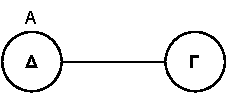
\includegraphics[scale = 0.9]{img/k1.pdf}
  \end{figure}
  Mi serve che:
  \[\Delta\nvDash \neg\neg A\mbox{ \textbf{o} }\Delta\vDash A,\,\,\,\forall
    \Delta\in G \mbox{ t.c. } \Gamma R\Delta\]
  Ma $\Delta\vDash A$ in quanto $A$ non vale in $\Gamma$ e $R$ è
  riflessiva, $\Gamma\nvDash A$. Ragiono ora su $\Delta\nvDash \neg\neg A$. Si
  ha però che $\Gamma\vDash \neg\neg A$, esistendo un $\Delta$ che rende vero
  $A$ (facendo i passaggi con la doppia negazione si arriva a voler cercare
  questo, devo avere che $\Gamma\nvDash\neg A$ e quindi che esiste almeno un
  $\Delta$ che verifica $A$), e quindi abbiamo dimostrato che: 
  \[\Gamma\nvDash\neg\neg A\to A\]
  Avendo un contro modello che verifica l'antecedente e non il conseguente
  dell'implicazione. 
\end{esempio}
\begin{esempio}
  Dimostriamo che intuizionisticamente:
  \[\Gamma\nvDash \neg\neg (A\lor B)\to \neg\neg A\lor \neg \neg B\]
  Il tableaux di questa formula non è chiuso.\\
  Vediamo che esiste un contromodello (le due rappresentazioni sono
  equivalenti(???)):  
  \begin{figure}[H]
    \centering
    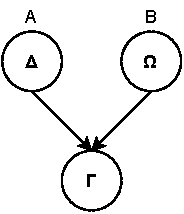
\includegraphics[scale = 0.9]{img/k2.pdf}
    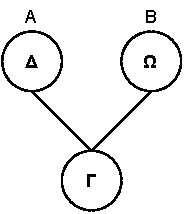
\includegraphics[scale = 0.9]{img/k3.pdf}
  \end{figure}
  Si ha quindi che $\Gamma$ è in relazione $R$ con se stesso, con $\Delta$, che
  a sua volta è in relazione solo con se stessa, e con $\Omega$, che è in
  relazione solo con se stessa. \\
  Partiamo con $\Gamma\vDash \neg\neg (A\lor B)$ che significa che esiste un
  nodo accessibile da $\Gamma$ in cui $A\lor B$ è vera. Questo è vero perché in
  $\Delta\vDash A$ e $\Omega\vDash B$ (ne basta uno dei due).\\
  Ora devo dimostrare che $\Gamma\nvDash\neg\neg A\lor \neg \neg B$ per avere
  che è un contromodello. Devo quindi avere che $\Gamma\nvDash \neg\neg A$ e
  $\Gamma\nvDash \neg\neg B$ in tutti i nodi accessibili da $\Gamma$. E vedo che
  in $\Delta$ non vale $B$ e in $\Omega$ non vale $A$, avendo quindi trovato il
  contromodello non potendo valere l'implicazione.
\end{esempio}
\subsection{Deduzione Naturale}
Introduciamo ora un nuovo calcolo, quello della \textbf{deduzione naturale},
introdotto da Gentzen negli anni '30 e perfezionato da Prawitz (perfezionamento
che tratteremo).\\
La deduzione naturale è un calcolo che è funzionale alla logica classica, alla
logica intuizionistica e alla logica minimale, con semplici variazioni nell'uso
delle regole.\\
La deduzione naturale è un calcolo la cui nozione di dimostrazione 'è molto
diversa dal calcolo a tableaux, che è un calcolo per refutazione (ovvero quando
vogliamo dimostrare una formula la segniamo $F$ e cerchiamo di ottenere una
configurazione chiusa ovvero una contraddizione), essendo quindi un calcolo
\textbf{indiretto e goal-oriented} ma che non permette di vedere come è fatta la
costruzione di una certa formula ma che dimostra che averla segnata $F$ porta d
avere un tableaux chiuso. Di contro la deduzione naturale utilizza, per
dimostrare una formula, un metodo diretto che, a partire da certe assunzioni,
costruisce la formula. Quindi l'ultimo passo di una dimostrazione in deduzione
naturale è la formula che si vuole dimostrare. \\
Con la scrittura
\[\bfrac{\pi}{A}\]
Diciamo che si è dimostrata la formula $A$ attraverso $\pi$, dove $\pi$ è un
insieme finito di passi, con eventuali assunzioni e applicazioni delle regole
della deduzione naturale.\\
Dire che $A$ è dimostrabile:
\[\vdash\bfrac{\pi}{A}\]
Significa dire che esiste una sequenza finita di applicazioni di regole e
assunzioni $\pi$ che termina con $A$ e quindi, non avendo alcuna formula a
sinistra di $\vdash$ si ha che la dimostrazione di $A$ non dipende da alcuna
formula e che in $\pi$ le eventuali assunzioni verranno chiuse, quindi sparendo,
rispetto alla deduzione di $A$ nei vari passi. Quindi $\vdash\bfrac{\pi}{A}$ è
il \textbf{frame} nel quale ci si muoverà.\\
La deduzione naturale comprende:
\begin{itemize}
  \item le \textbf{regole di introduzione}
  \item le \textbf{regole di eliminazione}
\end{itemize}
Date $A,B\in FBF$ si hanno:
\begin{table}[H]
  \Large
  \centering
  \begin{tabular}{c||c|c}
    connettivo& introduzione & eliminazione\\
    \hline
    \hline
    $\land$ & $\frac{A,B}{A\land B}i\land$&$\frac{A\land B}{A}e\land$
                                            $\frac{A\land B}{B}e\land$\\
    \hline
    $\lor$ &$\frac{A}{A\lor B}i\lor$
             $\frac{B}{A\lor B}i\lor$&$\frac{A\lor B,
                                       \bfrac{\bfrac{\cancel{A}}{\pi'}}{C},
                                       \bfrac{\bfrac{\cancel{B}}{\pi''}}{C}}{C}
                                       e\lor$\\
    \hline
    $\to$ & $\frac{\bfrac{\cancel{A}}
            {\bfrac{\pi}{B}}}{A\to B}i\to$ & $\frac{A,A\to B}{B}e\to$\\
    \hline
  \end{tabular}
\end{table}
Per l'eliminazione dell'or si ha che Prawitz ottiene questo risultato facendo:
\[\bfrac{\bfrac{A}{\pi'}}{C}\mbox{ e }\bfrac{\bfrac{B}{\pi''}}{C}\]
Ovvero se esiste una dimostrazione di $C$ che dipende solo da $A$ o $B$ sono
libero di dedurre $C$ tramite eliminazione dell'or \textbf{dimenticando},
specificata con $\cancel{X}$, le
assunzioni che ho separatemene di $A$ e di $B$, avendo $A\lor B$ come
assunzione: 
\[\frac{A\lor B,\bfrac{\bfrac{\cancel{A}}{\pi'}}{C},
    \bfrac{\bfrac{\cancel{B}}{\pi''}}{C}}{C}e\lor\]
tengo solo in considerazione la dimostrazione di $A\lor B$, quindi la scrittura
corretta è, qualora non sia quindi un'assunzione:
\[\frac{\bfrac{\pi}{A\lor B},\bfrac{\bfrac{\cancel{A}}{\pi'}}{C},
    \bfrac{\bfrac{\cancel{B}}{\pi''}}{C}}{C}e\lor\]
$C$ è una nuova formula che non è necessariamente contenuta in $A$ o $B$. Se non
si riesce a trovare questa $C$ non si può fare l'eliminazione dell'or.\\
Per l'inserimento dell'implicazione si suppone di fare un'assunzione $A$. Se
dopo un numero finito di applicazioni di regole $\pi$ otteno $B$ allora posso
introdurre l'implicazione $A\to B$. Si dice che la regola ``scarica''
l'assunzione $A$ e quindi indichiamo $\cancel{A}$. Quando scrivo poi
l'implicazione ho comunque che la dimostrazione non dipende più da $A$ perché è
già compresa in $A\to B$.\\
La regole di eliminazione dell'implicazione è detta \textbf{modus ponens}.\\
In merito all'implicazione ho che se ho un conseguente posso anche derivare
un'implicazione con qualsiasi antecedente, senza scaricare nulla:
\begin{gather*}
  \frac{^1\cancel{A},^2B}{}i\land\\
  \frac{A\land B}\land\\
  \frac{B}{A\to B}i\to\mbox{scaricando solo 1}
\end{gather*}
È quindi una semplificazione della regola di introduzione dell'implicazione.\\
\textbf{Queste regole sono valide sia per la logica classica che per quella
  intuizionistica che per quella modale.}\\
Dopo le regole dei tre connettivi binari abbiamo quelle per la costante del
\textit{falso}:
\begin{table}[H]
  \Large
  \centering
  \begin{tabular}{c||c|c}
    & introduzione & eliminazione\\
    \hline
    \hline
    $\bot$ & $\frac{A,\neg A}{\bot}i\bot$& $\frac{\bot}{B}e\bot$\\
    \hline
  \end{tabular}
\end{table}
L'eliminazione del falso mi ricorda che dal falso segue qualsiasi cosa. \\
\textbf{La regola dell'eliminazione del falso non si può usare in logica
  minimale}. \\
Possiamo quindi passare al connettivo unario della negazione:
\begin{table}[H]
  \Large
  \centering
  \begin{tabular}{c||c|c}
    & introduzione & eliminazione\\
    \hline
    \hline
    $\neg$ & $\frac{\bfrac{\bfrac{\cancel{A}}{\pi}}
             {\bot}}{\neg A}i\neg$& $\frac{\bfrac{\bfrac{\cancel{\neg A}}{\pi}}
             {\bot}}{ A}e\neg$\\
    \hline
  \end{tabular}
\end{table}
\textbf{La regola dell'introduzione del $\neg$ non si può usare in logica
  minimale}.\\
\textbf{La regola dell'eliminazione del $\neg$ non si può usare in logica
  intuizionistica}.\\
Questo calcolo, per $\neg$, è ``sovrabbondante'' rispetto alle regole in quanto
potrei riscrivere $\neg A$ come $A\to\bot$ ed eliminare le regole del
$\neg$. Per di più con questa implicazione Prawitz ha chiuso un problema aperto
che Gentzen, usando solo il $\neg$, non era riuscito a chiudere, ovvero il
\textbf{teorema di normalizzazione in logica intuizionistica con il calcolo
  della deduzione naturale}, dimostrando che tutte le dimostrazioni in deduzione
naturale possono essere normalizzate, ovvero ridotte ad una forma
\textit{normale}. \\
\textit{Gentzen ha chiamato questo calcolo deduzione naturale perché era
  fermamente convinto che questo fosse il modo di ragionare in matematica in
  modo ``naturale''.}\\
Vediamo quindi come costruire dimostrazioni in deduzione naturale, in una certa
logica. Anche in questo caso sintassi e semantica devono essere 
coerenti, ovvero formule valide nella logica data devono essere
dimostrabili con la deduzione naturale e formule non valide non devono essere
dimostrabili in nessun modo.\\
La prima difficoltà riguarda il come far partire la dimostrazione e questo è il
motivo per cui tutti i prover automatici per la deduzione naturale sono stati un
fallimento (mentre coi tableaux sappiamo sempre da dove partire).\\
\begin{definizione}
  Una dimostrazione $\vdash A$ di una formula $A$, in deduzione naturale, è una
  sequenza finita di applicazioni di regole, $\pi$, della deduzione naturale che
  termina con la formula $A$ e in cui eventuali assunzioni devono essere state
  tutte ``scaricate'', essendo quindi chiusa rispetto alle assunzioni:
  \[\bfrac{\pi}{A}\]
  Se $A$ è dimostrabile da un insieme di formule $A_1,\ldots A_n$ di premesse
  allora in $\pi$ possono rimanere assunte $A_1,\ldots A_n$. Questo si indica
  con:
  \[A_1,\ldots A_n\vdash A\]
\end{definizione}
Vediamo qualche esempio.
\begin{esempio}
  Il primo esempio è quello del terzo escluso in logica classica (vedendo anche
  perché non vale in logica intuizionistica).\\
  Con $\vdash_{CL}$ indichiamo che una cosa è dimostrabile in logica
  classica. Vogliamo quindi dimostrare che:
  \[\vdash_{CL}A\lor \neg A\]
  Numeriamo le assunzioni, per poter indicare accanto alla regola che scarica
  l'assunzione il suo numero:
  \begin{enumerate}
    \item $A$
    \item $\neg(A\lor \neg A)$
  \end{enumerate}
  Procedo quindi:
  \[\frac{^1A}{A\lor \neg A}i\lor\]
  Potremmo pensare di aver finito, avendo ottenuto la formula, ma non è
  così. Dobbiamo infatti scaricare l'assunzione $A$. Assumo quindi un'altra
  assunzione, la 2 e procedo:
  \[\frac{^2\neg(A\lor \neg A), A\lor \neg A}{\bot}i\bot\]
  Ma dal falso posso dire che segue qualsiasi cosa in logica classica e quindi,
  iniziando a scaricare l'assunzione 1:
  \[\frac{\bot}{\neg A}i\neg\]
  Quindi, nel complesso ho:
  % {\Large{\[\frac{^1\cancel{A}}{\frac{^2\neg(A\lor \neg A), A\lor \neg
  %   A}{\frac{\bot}{\neg A}i\neg}i\bot}i\lor\]}}
  \begin{gather*}
    \frac{^1\cancel{A}}{}i\lor\\
    \frac{^2\neg(A\lor \neg A), A\lor \neg A}{}i\bot\\
    \frac{\bot}{\neg A}i\neg
  \end{gather*}
  Devo ancora scaricare la 2. Continuo:
  \[\frac{\neg A}{A\lor \neg A}i\lor\]
  Ma devo ancora scaricare la 2. Assumo quindi nuovamente la 2:
  \[\frac{^2\neg(A\lor \neg A), A\lor \neg A}{\bot}i\bot\]
  E quindi:
  \[\frac{\bot}{\neg \neg(A\lor \neg A)}i\neg\]
  che scarica 2, avendo complessivamente:
  % {\Large{\[\frac{^1\cancel{A}}{\frac{^2\cancel{\neg(A\lor \neg A)}, A\lor \neg
  %           A}{\frac{\bot}{\frac{\neg A}{\frac{^2\cancel{\neg(A\lor \neg A)},
  %                 A\lor \neg A}{\frac{\bot}{\neg \neg(A\lor \neg
  %                   A)}i\neg}i\bot}i\lor}i\neg}i\bot}i\lor\]} }
  \begin{gather*}
    \frac{^1\cancel{A}}{}i\lor\\
    \frac{^2\cancel{\neg(A\lor \neg A)}, A\lor \neg A}{}i\bot\\
    \frac{\bot}{}i\neg\\
    \frac{\neg A}{}i\lor\\
    \frac{^2\cancel{\neg(A\lor \neg A)}, A\lor \neg A}{}i\bot\\
    \frac{\bot}{\neg \neg(A\lor \neg A)}i\neg
  \end{gather*}

 % \end{equation*}
  Ma sono arrivato alla doppia negazione del principio del terzo escluso e non
  al terzo escluso. Finora ho usato solo regole valide anche in logica
  intuizionistica, che indico con $INT$ e quindi la doppia negazione del terzo
  escluso è dimostrabile 
  in logica intuizionistica, avendo scaricato tutte le assunzioni e avendo usato
  regole valide in quella logica:
  \[\vdash_{INT}\neg \neg(A\lor \neg A)\]
  Ovviamente la doppia negazione del terzo
  escluso vale anche in logica classica per lo stesso ragionamento.\\
  Voglio però arrivare al terzo escluso in logica classica. Per scaricare la 2
  posso fare eliminazione del \textit{false} (che non vale in logica
  intuizionistica ma solo in logica classica):
  \[\frac{\bot}{A\lor \neg A}e\bot\]
  che consuma la 2:
  \begin{gather*}
    \frac{^1\cancel{A}}{}i\lor\\
    \frac{^2\cancel{\neg(A\lor \neg A)}, A\lor \neg A}{}i\bot\\
    \frac{\bot}{}i\neg\\
    \frac{\neg A}{}i\lor\\
    \frac{^2\cancel{\neg(A\lor \neg A)}, A\lor \neg A}{}i\bot\\
    \frac{\bot}{A\lor \neg A}e\bot
  \end{gather*}
  arrivando quindi a:
  \[\vdash_{CL}A\lor \neg A\]
  Che non è dimostrabile in logica intuizionistica (come già si sapeva).
\end{esempio}
\begin{esempio}
  Vediamo una delle formule di De Morgan:
  \[\vdash_{INT}\neg(A\lor B)\to \neg A\land \neg B\]
  Come assunzioni ho:
  \begin{enumerate}
    \item $\neg (A\lor B)$
    \item $A$
    \item $B$
  \end{enumerate}
  Parto dal basso, sapendo che vorrei ottenere:
  \[\frac{\neg A\land \neg B}{\neg(A\lor B)\to \neg A\land \neg B}i\to\mbox{
      (scaricando 1)}\]
  Vediamo i passaggi i passaggi ``risalendo'', procedendo, come si dice, ``per
  necessità'' (ricostruendo ogni volta ciò che mi serve risalendo nella
  dimostrazione, ricostruendola a ritroso): 
  \begin{gather*}
    \frac{^2\cancel{A}}{}i\lor \mbox{, } \frac{^3\cancel{B}}{}i\lor\\
    \frac{A\lor B, ^1\cancel{\neg (A\lor B)}}{}i\bot \mbox{, } \frac{A\lor
      B,^1\cancel{\neg (A\lor B)}}{}i\bot\\  
    \frac{\bot}{}i\neg \mbox{(scaricando 2), }\frac{\bot}{}i\neg\mbox{
      (scaricando 3)}\\ 
    \frac{\neg A, \neg B}{}i\land\\
    \frac{\neg A\land \neg B}{\neg(A\lor B)\to \neg A\land \neg B}i\to\mbox{
      (scaricando 1)}
  \end{gather*}
  Chiudendo la dimostrazione avendo scaricato tutto ed essendo arrivati alla
  formula voluta. L'unico passo ``strano'', era capire che $\neg A/B$ era in
  contraddizione con $A/B$, portando all'introduzione dell'or e poi del
  $\bot$.\\
  Vediamo un'altra dimostrazione della stessa:
  \[\vdash_{INT}\neg(A\lor B)\to \neg A\land \neg B\]
  Assumo:
  \begin{enumerate}
    \item $A$
    \item $\neg(A\lor B)$
    \item $B$
  \end{enumerate}
  Procediamo quindi con la dimostrazione:
  \begin{gather*}
    \mbox{Ho }\pi_1 =\\
    \frac{ ^1\cancel{A}}{}i\lor\\
    \frac{A\lor B, ^2\cancel{\neg(A\lor B)}}{}i\bot\\
    \frac{\bot}{\neg A}i\neg\mbox{(scaricando 1)}\\
    \mbox{rifaccio anche con B, avendo} \pi_2=\\
    \frac{ ^3\cancel{B}}{}i\lor\\
    \frac{A\lor B, ^2\cancel{\neg(A\lor B)}}{}i\bot\\
    \frac{\bot}{\neg B}i\neg\mbox{(scaricando 3)}\\
    \mbox{sono nella situazione}\\
    \frac{\pi_1, p_2}{}i\land\\
    \frac{\neg A \land \neg B}{\neg(A\lor B)\to \neg A\land \neg
      B}i\to\mbox{(scaricando 2)}  
  \end{gather*}
  (i passaggi di $\pi_1$ e $\pi_2$ li avrei potuti scrivere uno accanto
  all'altro). \\
  Quindi, avendo usato solo regole valide per la logica intuizionistica:
  \[\vdash_{INT}\neg(A\lor B)\to \neg A\land \neg B\]
  Passiamo alla dimostrazione della conversa:
 \[\vdash_{INT}\neg A\land \neg B\to\neg(A\lor B)\]
 Sappiamo già che il tableaux non chiude.\\
 Assumo:
 \begin{enumerate}
   \item $\neg A\land \neg B$
   \item $A\lor B$
   \item $A$
   \item $B$
 \end{enumerate}
 Procediamo quindi con la dimostrazione:
 \begin{gather*}
   \frac{^1\cancel{1\neg A\land \neg B}}{}e\land\mbox{, }\frac{^1\cancel{1\neg
         A\land \neg B}}{}e\land\\ 
   \frac{\neg A, ^3 \cancel{A}}{}i\bot\mbox{, }\frac{\neg B,
     ^4\cancel{B}}{}i\bot\\  
   \frac{\bot,\bot,^2\cancel{A\lor B}}{}e\lor\mbox{(scaricando 3 e 4)}\\
   \frac{\bot}{}i\neg\mbox{(scaricando 2)}\\
   \frac{\neg(a\lor B)}{\neg A\land \neg B\to\neg(A\lor B)}i\to\mbox{(scaricando
     1)} 
 \end{gather*}
 Ho quindi dimostrato, nel complesso, un'equivalenza avendo entrambi i versi
 dell'implicazione (e per entrambi i versi si ha un tableaux chiuso), sia in
 logica classica che intuizionistica.  
\end{esempio}
\begin{esempio}
  Proviamo a dimostrare l'altra formula di De Morgan:
  \[\vdash_{INT}\neg(A\land B)\to \neg A\lor \neg B\]
  Il tableaux della formula non chiude quindi arriveremo a dire che:
  \[\nvdash_{INT}\neg(A\land B)\to \neg A\lor \neg B\]
  Siano date le seguenti assunzioni:
  \begin{enumerate}
    \item $A$
    \item $B$
    \item $\neg(A\land B)$
  \end{enumerate}
  Procediamo quindi con la dimostrazione:
  \begin{gather*}
    \frac{^1\cancel{A},^2B}{}i\land\\
    \frac{A\land B, ^3\cancel{\neg(A\land B)}}{}i,\bot\\
    \frac{\bot}{}i\neg\mbox{(scaricando 1)}\\
    \frac{\neg A}{}i\lor\\
    \frac{\neg A \lor \neg B}{}i\to\mbox{(scaricando 3)}\\ 
    \frac{\neg(A\land B)\to\neg A\lor \neg B}{}
  \end{gather*}
  Ma non si è scaricato $B$ e quindi non è una dimostrazione, né classica né
  intuizionistica.\\
  Vediamo se la conversa vale intuizionisticamente:
  \[\vdash_{INT}\neg A\lor \neg B\to\neg(A\land B)\]
  Assumo:
  \begin{enumerate}
    \item $\neg A\lor \neg B$, ovvero assumo l'antecedente
    \item $\neg A$
    \item $\neg B$
    \item $A\land B$
  \end{enumerate}
 Procediamo quindi con la dimostrazione:
 \begin{gather*}
    \frac{ ^4\cancel{A\land B}}{}e\land\mbox{, }
    \frac{ ^4\cancel{A\land B}}{}e\land\\
    \frac{A, ^2\cancel{\neg A}}{}i\bot\mbox{, }
    \frac{B,^3\cancel{\neg B}}{}i\bot\\
    \frac{\bot, ^1\cancel{\neg A\lor \neg B}}{}e\lor\mbox{(scaricando 2 e 3)}\\
    \frac{\bot}{}i\neg\mbox{(scaricando 4)}\\
    \frac{\neg (A\land B)}{\neg A\lor \neg B\to\neg(A\land
      B)}i\to\mbox{(scaricando 1)} 
  \end{gather*}
  Quindi, avendo usato solo regole valide per la logica intuizionistica:
  \[\vdash_{INT}\neg A\lor \neg B\to\neg(A\land B)\]
  Quindi ``mezza'' De Morgan vale in logica intuizionistica.
\end{esempio}
\noindent
\textbf{Durante la lezione 6, parte 2, altri esempi di dimostrazione}:
\begin{itemize}
  \item $\vdash_{INT}(A\to\neg B)\to(B\to \neg A)$
  \item $\vdash_{INT}(\neg A\lor\neg B)\to(B\to \neg A)$
  \item $\vdash_{INT}(A\to(B\to C))\to(B\to(A\to C)$, detta \textbf{scambio
    degli antecedenti}  
  \item $\nvdash_{INT} ((A\to B)\to A)\to A$, detta \textbf{legge di Peirce},
  che vale solo in logica classica
  \item $\nvdash_{INT}(A\to B)\iff(\neg B\to \neg A)$, detta \textbf{legge di
    contrapposizione}, che ricorda il\textbf{ teorema di deduzione della logica
    classica} che legava dimostrabilità e implicazione, avendo a livello
  proposizionale che se con ipotesi $A$ dimostro $B$, $A\vdash B$ allora $A\to
  B$. Classicamente si ha anche che $\vdash \neg B\to \neg A$ se $A\vdash B$ e
  si noti che è il procedimento di una \textit{dimostrazione per assurdo},
  secondo la logica classica. Vale in logica classica ma il $\gets$ non vale in
  logica intuizionistica. \textbf{Non posso dimostrare direttamente per assurdo
    in logica intuizionistica} ma si usano dei ``meta-sistemi''
  \item $\vdash_{INT}((((A\to B)\to A)\to A)\to B)\to B$
\end{itemize}
\textbf{Se la formula è un'implicazione si assume spesso l'antecedente che poi
  si scarica all'ultimo passo.} Non si hanno comunque strategie
deterministiche.\\
Si è notato come non ci sia un metodo preciso per ottenere la strategia e per di
più la strategia non è unica potenzialmente. Nel primo esempio si parte
dall'alto, nel secondo dal basso.\\
Per capire se esiste una dimostrazione faccio prima la prova coi tableaux, che
se chiude mi garantisce l'esistenza di una dimostrazione.\\
L'idea di partire a dimostrare sapendo a quali connettivi bisogna arrivare sia
adatta molto bene anche la \textbf{calcolo dei sequenti} di Gentzen (sono un
calcolo diretto), dove si
parte sempre dal basso, risalendo ``per necessità'', fino ad arrivare agli
assiomi caratteristici della logica in uso e del calcolo dei sequenti. Si hanno
meccanismi di traduzione da tableaux intuizionistici a sequenti e da sequenti a
deduzione logica (???). I sequenti sono ``mediani'' nel paradigma del
goal-oriented. \\
Anche in deduzione naturale, in modo analogo alla matematica, si possono usare i
\textbf{lemmi}.
\begin{esempio}
  Dimostriamo:
  \[\vdash_{INT}\neg\neg (A\land B)\to \neg\neg A\land \neg \neg B\]
  Si assume:
  \begin{enumerate}
    \item $\neg A$
    \item $\neg\neg(A\land B)$
    \item $\neg B$
  \end{enumerate}
  Di ha quindi la dimostrazione:
  \begin{gather*}
    \frac{^1 \cancel{\neg A}}{}i\lor \mbox{, }
    \frac{^3 \cancel{\neg B}}{}i\lor\\
    \frac{\neg A\lor \neg B}{\rule{49pt}{0.4pt}}\mbox{regola derivata, }
    \frac{\neg A\lor \neg B}{\rule{49pt}{0.4pt}}\mbox{regola derivata}\\
    \frac{\neg (A\land B),^2\cancel{\neg\neg(A\land B)}}{}i\bot\mbox{, }
    \frac{\neg  (A\land B),^2\cancel{\neg\neg(A\land B)}}{}i\bot\\ 
    \frac{\bot}{}i\neg\mbox{(scaricando 1), }
    \frac{\bot}{}i\neg\mbox{(scaricando 3)}\\ 
    \frac{\neg\neg A, \neg\neg B}{}i\land\\
    \frac{\neg\neg A\land \neg\neg B}{\neg\neg (A\land B)\to \neg\neg a\land
      \neg \neg B}i\to \mbox{(scaricando 2)}
  \end{gather*}
  con la doppia barra indico una regola derivata da un precedente lemma (nel
  nostro caso dalla legge/teorema di De Morgan) che quindi chiamiamo lemma di De
  Morgan, non dovendo quindi dimostrare nuovamente la cosa, riducendo la
  ``complessità'' della dimostrazione.
\end{esempio}
Comunque non si hanno strategie deterministiche per iniziare una dimostrazione,
si hanno comunque suggerimenti in base alla formula, ad esempio se ho una cosa
del tipo $A\to B$ si parte spesso, ma non sempre, assumendo $A$ per poi cercare
di scaricarla. Bisogna sempre prima guardare bene la formula che si deve
dimostrare, ragionando su sottoformule etc$\ldots$
\subsection{Ottimizzazione dei Tableaux}
Parliamo ora di \textbf{ottimizzazione dei tableaux intuizionistici}.\\
\begin{esempio}
  Riprendiamo il tableaux di Fitting per la doppia negazione del terzo escluso:
  \[F\neg \neg (A\lor \neg A)\]
  che ricordiamo dimostrabile in logica intuizionistica per il teorema di
  Kolmogorov-Glivenko. \\
  Riprendiamo il tableaux di Fitting:
  \begin{gather*}
    \frac{F\neg \neg (A\lor \neg A)}{}\\
    \frac{T\neg(A\lor \neg A)}{}\\
    \frac{FA\lor \neg A}{}\\
    \frac{FA,F\neg A}{TA}
  \end{gather*}
  Che sembra non chiudere. \\
  Si ricorda però che, sempre Fitting, risolve la questione ripetendo una
  formula: 
  \begin{gather*}
    \frac{F\neg \neg (A\lor \neg A)}{}\\
    \frac{T\neg(A\lor \neg A)}{}\\
    \frac{FA\lor \neg A, T\neg(A\lor \neg A)}{}\\
    \frac{FA,F\neg A,T\neg(A\lor \neg A)}{}\\
    \frac{TA,T\neg(A\lor \neg A)}{}\\
    \frac{TA, FA\lor \neg A}{TA, FA, F\neg A}
  \end{gather*}
  che chiude.\\
  Si è usato il fatto che si è usata, come regola per il $T$ di $\neg$:
  \[\frac{S, T\neg A}{S, FA, T\neg A}\]
\end{esempio}
Nell'esempio ci si è rifatti al concetto di \textbf{realizzabilità}.
\begin{definizione}
  Preso un nodo $\Gamma$ di un modello di Kripke per la logica intuizionistica
  diremo che $\Gamma$ \textbf{realizza} $TA$ sse $\Gamma$ \textup{forza} $A$,
  ovvero sse: 
  \[\Gamma\vDash A\]
  Inoltre si ha che $\Gamma$ \textbf{realizza} $FA$ sse in $\Gamma$ \textbf{non
    è vera} $A$, ovvero sse:
  \[\Gamma\nvDash A\]
  Abbiamo quindi legato il segno $T/F$ al \textbf{forcing intuizionista}. Le
  regole devono quindi mantenere la realizzabilità.
\end{definizione}
Vediamo, sempre pensando all'esempio, cosa significhi mantenere la
realizzabilità parlando di $T\neg A$. Si ha che, intuizionisticamente:
\[\Gamma\vDash \neg A\]
Ma nell'intuizionismo significa che:
\[\forall\Delta \mbox{ t.c }\Gamma R \Delta, \Delta\nvDash A\]
Se diciamo che una formula realizzata prima di applicare una regola deve essere
realizzata anche dopo tale applicazione si ha che, avendo:
\[\frac{S, T\neg A}{S, FA, T\neg A}\]
$FA$ può essere eliminata, quindi restringendo $S$ a $S_C$ non è più garantito
che sia realizzato $FA$ ovvero che sia forzata $A$. Dato che questo deve
avvenire $\forall\Delta$ mi ``porto dietro'' $T\neg A$ in modo che in ogni punto
del tableaux sia realizzabile la formula $\neg A$ (ma questo succede solo se
ripeto il $T$).\\
Non sempre bisogna ripetere la $T$, ad esempio:
\[\frac{S, T(A\land B)}{S, TA, TB}\]
che passando da una $T$ a due $T$ non crea problemi anche se restringo a
$S_T$, avendo un $\Gamma$ che realizza $TA$ e $TB$ allora ho che forza $A\land
B$.\\
Vale lo stesso discorso anche avendo:    
\[\frac{S, T(A\lor B)}{S, TA/S, TB}\]
garantendo o da un alto o dall'altro la realizzabilità di $A\lor B$. Infatti se
è 
realizzato $TA$ ho un $\Gamma$ che forza $A$ e che automaticamente forza $A\lor
B$. Viceversa con $TB$ ho un $\Gamma$ che forza $B$ e che automaticamente forza
$A\lor B$.\\
Abbiamo un'altra regola che obbliga a ripete:
\[\frac{S, T(A\to B)}{S, FA, T(A\to B)/S, TB}\]
Dove, avendo che $FA$ può essere ``tagliato'' da una restrizione $S_T$ nel primo
branch, conservo anche la formula (non avendo $F$ nel secondo branch non devo
ripetere). \\
Vediamo un calcolo che, ``modulo backtracking'', non necessiterà della
ripetizione delle formule, avendo già tutta la sua semantica all'interno del
calcolo. Si parla quindi di \textbf{semantic tableaux}, avendo che i tableaux
``mimano'' la semantica della logica di riferimento. Più semantica
incorporariamo nelle regole stesse e migliore sarà il calcolo dal punto di vista
dell'efficienza.\\
Quanto detto viene bene con il $T$ di $\neg$.\\
Aggiungiamo a $T$ e $F$ il segno $F_C$ che significa \textbf{falso certo}:
\begin{table}[H]
  %\large
  \centering
  \begin{tabular}{c||c|c|c}
    & {\small{$T$-regola}}& {\small{$F$-regola}} & {\small{$F_C$-regola}}\\
    \hline
    \hline
    $\land$ & $T\land=\frac{S,T(A\land B)}{S,TA,TB}$&
              $F\land=\frac{S,F(A\land B)}{S,FA/S,FB}$&
              $F_C\land=\frac{S,F_C(A\land B)}{S_C,F_CA/S_C,F_CB}$\\ 
    \hline
    $\lor$ & $T\lor=\frac{S,T(A\lor B)}{S,TA/S,TB}$&
                        $F\lor=\frac{S,F(A\lor B)}{S,FA,FB}$&
                        $F_C\lor=\frac{S,F_C(A\lor B)}{S,F_CA,F_CB}$\\
    \hline
    $\to$ & $T\to=\frac{S,T(A\to B)}{S,FA, T(A\to B)/S,TB}$&
                        $F\to=\frac{S,F(A\to B)}{S_C,TA,FB}$&
                        $F_C\to=\frac{S,F_C(A\to B)}{S_C,TA,F_CB}$\\
    \hline
    $\neg$ & $T\neg=\frac{S,T(\neg A)}{S,F_CA}$&
                        $F\neg=\frac{S,F(\neg A)}{S_C,TA}$&
                        $F_C\neg=\frac{S,F_C(\neg A)}{S_C,TA}$\\
    \hline
  \end{tabular}
\end{table}
Il nuovo segno è dato in quanto al semantica del $\neg$ ci dice che, avendo il
forcing di $\neg A$, $A$ deve rimanere falso in ogni nodo del modello di Kripke
e quindi è un falso che deve permanere sempre in tutto il tableaux.\\
$S_C$ è definito come l'insieme $S$ meno l'insieme delle formule segnate con
$F$ (detto $FC_J$): 
\[S_C=S-\{FC_j\}\]
Notiamo, in prima istanza, come da formule $F_C$ otteniamo sempre formule $F_C$
o $T$, stabilizzando il tableaux.\\
Nell'implicazione di $F_C$ notiamo ancora però la presenza di $TA$ che
porterebbe a fare lo stesso ragionamento di replicazione della formula
dell'implicazione ma questo è uno step successivo di ottimizzazione.\\
Un tableaux in questo nuovo calcolo è chiuso secondo le regole dei normali
tableaux ma anche se ho $TA,F_CA$.
\begin{esempio}
  Riprendiamo la doppia negazione del terzo escluso con questo nuovo calcolo:
  \begin{gather*}
    \frac{F\neg \neg (A\lor \neg A)}{}\\
    \frac{T\neg(A\lor \neg A)}{}\\
    \frac{F_C (A\lor\neg A)}{}\\
    \frac{F_C A, F_C\neg A}{}\\
    \frac{F_C A, TA}{}
  \end{gather*}
  e quindi il tableaux è chiuso, anche senza aver ripetuto il $T\neg$.
\end{esempio}
\textbf{$F_C$ è stato proposto da Moscato a Fitting ed è stato accolto nello
  studio dell'intuizionismo}.\\
Si è quindi incorporato più semantica nel calcolo infatti:
\[\Gamma\vDash F_CA \iff \Gamma\vDash \neg A\]
avendo che la semantica del $\neg$ viene incorporata dal segno $F_C$, avendo che
$\Gamma$ realizza $F_C A$ sse realizza $\neg A$. Abbiamo fatto quindi un primo
step di ottimizzazione.\\
Dal punto di vista ``proof teoretico'' il segno $F_C$ riesce a evitare
duplicazioni della formula $\neg A$, a livello intuizionista, che sarebbero
sempre necessarie per chiudere il tableaux.\\
Ripariamo dalla doppia negazione del terzo escluso:
\[\neg\neg(A\lor \neg A)\]
Si ha, con il nuovo calcolo:
\begin{gather*}
  \frac{F\neg\neg(A\lor \neg A)}{}\\
  \frac{T\neg (A\lor \neg A)}{}\\
  \frac{F_c(A\lor\neg A)}{}\\
  \frac{F_C A, F_C\neg A}{F_C A, TA}
\end{gather*}
Avendo che il tableaux chiude (senza il ragionamento di Fitting di ripetere le
formule).
Il discorso può essere generalizzato dicendo che, ogni volta che si vuole
applicare il teorema di Kolmogorov-Glivenko, ragionando come Fitting avrò sempre
bisogno di ripetere formule, avendo in partenza una doppia negazione (dovendo
fare comunque un $F\neg$ e un $T\neg$ come prime mosse, se non uso
$F_C$). Quindi, avendo una formula valida classicamente, per dimostrare
intuizionisticamente la doppia negazione, posso usare $F_C$ evitando la
ripetizione di formule, a meno di avere poi nella formula dei $T\to$. Si ha
quindi un \textbf{trattamento ottimale} del $T\neg$ ma manca quello di
$T\to$. \\
Moscato, coi vari collaboratori, ha lavorato anni per trovare una
soluzione soddisfacente, quindi un calcolo corretto e completo, che rimuovesse
anche la ripetizione del $T\to$. Si sono quindi chiesti se, a livello
proposizionale, esistesse una soluzione al problema. Si arriverà a dire che c'è
una soluzione a livello proposizionale ma non a livello predicativo (il
$T\forall$ richiede sempre e comunque la ripetizione) e
nemmeno a livello di logica classica (lato predicativo si ha ripetizione sia per
$T\forall$ che per $T\exists$). Nella logica classica, lato proposizionale, vale
quindi la regola di Chruch-Rosser e quindi non sarà mai necessario ripetere una
formula mentre in logica intuizionistica questo non vale e quindi bisogna
pensare a delle strategie per evitarlo. Il calcolo puro di Fitting prevede per
forza ripetizioni per $\neg$ e $T\to$ ma in questo nuovo calcolo con $F_C$ ho
solo ripetizioni per $T\to$.\\ 
Presentiamo quindi un ulteriore calcolo che rimuova anche questa ripetizione.\\
Che nuovo calcolo proviene da un'idea di Dikov, che aveva ragionato sulla
deduzione naturale e sul calcolo dei sequenti di Gentzen. Dikov aveva studiato
cosa succede a livello di deduzione naturale quando si assumono nuovamente certe
formule, costruendo un calcolo in cui non succede. Moscato e Miglioli, studiando
il lavoro di Dikov, hanno cercati di applicare le stesse regole al calcolo a
tableaux ottimizzato. \\
L'idea è di studiare in modo approfondito come è fatto l'antecedente
dell'implicazione e non dare una sola regola per il $T\to$ ma dare tante regole
a seconda della forma dell'antecedente dell'implicazione.\\
Si va quindi ad analizzare la formula del tipo:
\[T\,\, A\to B\]
Si studia l'antecedente $A$. Si hanno quindi vari casi:
\begin{itemize}
  \item $A$ è atomica o negata, che indico con $AN$ (per dire $A$ e Negata)
  \item $A$ è una disgiunzione, quindi del tipo $A=C\lor D$
  \item $A$ è una congiunzione, quindi del tipo $A=C\land D$
  \item $A$ è un'implicazione, quindi del tipo $A\to B$
\end{itemize}
Si da quindi una regola ad hoc per ciascuna tipologia di antecedente. Si hanno
quindi quattro formule.\\
Facciamo qualche considerazione preliminare. In primis si nota come il calcolo
venga ancora più complicato, complicando il lavoro di un prover, anche se questo
è trascurabile dal punto di vista computazionale. Una seconda osservazione è che
non si riesce a trovare un modo per importare nel calcolo la semantica
dell'implicazione, come per il caso di $T\neg$, che importava la semantica della
negazione intuizionistica nel calcolo. Questa infatti è un'idea più
\textit{sintattica} e sostituisce una formula con un suo equivalente
intuizionista, che abbia nell'antecedente una complessità implicazionale sempre
più bassa, fino ad arrivare a formule atomiche o negate per poter applicare la
regola di base, avendo che la regola per le atomiche e le negate non prevede
ripetizioni di formule. Si ha quindi una ``trasformazione di formule''. Si
ottiene un calcolo privo di ripetizioni,\textit{ anche se può darsi che esista
  una soluzione più semantica e meno sintattica del problema di questo tipo di
  calcolo, magari cercando un nuovo segno ad hoc}. \\
Vediamo quindi queste 4 regole che sostituiscono la precedente regola per
$T\to$: 
\begin{table}[H]
  \Large
  \centering
  \begin{tabular}{c|c}
    & $\mathbf{T\to}$\\
    \hline
    $Ant=A$ \textit{o} $Ant=\neg A$ & $\frac{S,TA\to B}{S,FA/S,TB}T\to AN$\\
    \hline
    $Ant=A\land B $ & $\frac{S,T(A\land B)\to C}{S,T(A\to(B\to C))}T\to \land$\\
    \hline
    $Ant=A\lor B$ & $\frac{S,T(A\lor B)\to C}{S,TA\to C, TB\to C}T\to \lor$\\
    \hline
    $Ant =A\to B$ & $\frac{S,T(A\to B)\to C}{S, FA\to B, TB\to C/S, TC}T\to \to$\\
    \hline
  \end{tabular}
\end{table}
Si nota che la complessità logica di $B$ non ha importanza. In tutti i casi si
ottengono complessità implicazionali minori, avendo antecedenti sempre meno
complessi logicamente nella risultante rispetto alla premessa.\\
Questo nuovo calcolo, con questa nuova regola per $T\to$ è \textbf{corretto,
  completo e senza ripetizioni}.\\
A livello di prover questo risultato permette di non dover creare liste
aggiuntive di formule da ripetere (considerando che Fitting nemmeno limitava la
cosa a $T\neg $ e $T\to$).
\begin{esempio}
  Studiamo:
  \[\vdash_{INT} ((\neg A\lor \neg \neg A)\to A)\to A\]
  \begin{gather*}
    \frac{F ((\neg A\lor \neg \neg A)\to A)\to A}{}F\to\\
    \frac{T(\neg A\lor \neg \neg A)\to A, FA}{}T\to\lor\\ 
    \frac{T\neg A\to A, T\neg\neg A\to A,FA}{}T\to AN\\
    \frac{T\neg A\to A, F\neg\neg A, FA/T\neg A\to A, TA,FA}{}F\neg\mbox{(chiude
      branch destro)}\\ 
    \frac{T\neg A\to A,T\neg A}{}T\neg\\
    \frac{T\neg A\to A,F_C A}{}T\to AN\\
    \frac{F\neg A, F_CA/TA,F_CA}{}F\neg\mbox{(chiude branch destro)}\\
    TA, F_CA
  \end{gather*}
  Avendo che il tableaux chiude, senza ripetizioni.\\
  Si nota che avendo $T\neg A\to A, T\neg\neg A\to A,FA$ si osserva che è
  prodotto da un antecedente in $\lor$ con due negate. Si hanno quindi ora due
  antecedenti entrambi con due negate, sotto $T$, che mi riportano alla regola
  per il $T\to$ delle atomiche e delle negate.
\end{esempio}
Dimostreremo che questo calcolo è corretto e completo.\\
Il prover PTP è basato su questo calcolo con ulteriori strategie di
ottimizzazione. \\
Possiamo quindi vedere la dimostrazione del teorema di Kolmogorov-Glivenko, che
riscriviamo per comodità, tramite il calcolo a tableaux con $F_C$ e la non
ripetizione di $T\neg$ e $T\to$.
\begin{teorema}[Teorema di Kolmogorov-Glivenko]
  Se una formula $A$ è dimostrabile in logica classica allora e solo allora è
  dimostrabile in logica intuizionistica la doppia negazione di tale formula, a
  livello proposizionale. Formalmente si ha quindi:
  \[\vdash_{CL} A \iff \vdash_{INT}\neg\neg A\]
  Quindi tutte le tesi classiche sono dimostrabili, se doppiamente negate, in
  logica intuizionistica.
\end{teorema}
\begin{proof}
  Per fare la dimostrazione si introduce una nuova regola:
  \[\frac{S, TA\to B}{S,F_CA/S_C, TB}\overline{T\to}\]
  che chiamiamo appunto $T\to$ soprassegnato. Questa regola è corretta dal punto
  di vista del calcolo intuizionistica e possiamo usarla quando vogliamo. La sua
  peculiarità rispetto all'originale $T\to$ è che nel branch a sinistra ho $F_C
  A$ quindi non si avrà mai il taglio della stessa applicando regole
  intuizionistiche. Nel branch di destra si ha $TB$ che già non verrebbe mai
  tagliata ama, per correttezza e non per completezza, si restringe $S$ a
  $S_C$.\\
  Ricordiamo che la vecchia regola era, dove si ripeteva la formula a causa di
  $FA$ nel branch di sinistra e non si restringeva $S$ in quello di destra:
  \[\frac{S, TA\to B}{S,FA, TA\to B/S, TB}T\to\]
  La $\overline{T\to}$ è una versione corretta ma non completa di $T\to$. L'uso
  della prima quindi comporta un calcolo corretto ma non completo, mentre la
  seconda sia corretto che completo.\\
  Ora a noi basta avere una formula corretta, cosa che rende possibile il
  poterla applicare ogni volta che voglio.\\
  Parto quindi dal tableaux intuizionista di $\neg\neg A$:
  \begin{gather*}
    \frac{F\neg\neg A}{}F\neg\\
    \frac{T\neg A}{F_C A}T\neg
  \end{gather*}
  Avendo che da questo momento in poi il tableaux intuizionista diventa
  equivalente a quello classico, con solo i segni $T$ e $F_C$. Dobbiamo
  dimostrarlo per casi, a seconda della natura di $A$:
  \begin{itemize}
    \item $A$ è una formula atomica quindi se chiude classicamente $F_CA$ chiude
    anche intuizionisticamente
    \item $A$ è del tipo $B\lor C$, avendo che $F_C (B\lor C)$ produce/deduce
    $F_CB,F_CC$
    \item $A$ è del tipo $B\land C$, avendo che $F_C (B\land C)$ produce/deduce
    $F_CB/F_CC$
    \item $A$ è del tipo $\neg B$, avendo che $F_C \neg B$ produce/deduce $TB$
    \item $A$ è del tipo $B\to C$, avendo che $F_C (B\to C)$ produce/deduce
    $TB,F_CC$
  \end{itemize}
  Analizzo l'ultimo caso, avendo $TB,F_CC$. Questo è l'unico caso in cui potrei
  avere 
  ancora formule che vengono tagliate con le regole intuizionistiche, in caso di
  implicazione ma posso evitare la cosa. Infatti, se $TB$ fosse anch'essa
  un'implicazione, potrei usare il $\overline{T\to}$ e ottenere formule che non
  verranno mai tagliate dall'applicazione di regole intuizionistiche, avendo che
  il tableaux classico e quello intuizionistico coincidono. Ne segue che se
  quello classico chiude allora chiude anche quello intuizionistico. Il trucco
  sta nel $F_CA$ nel branch sinistro del risultante della regola del
  $\overline{T\to}$, vale a dire rafforzare, scrivendo $F_C$ invece di $F$
  della'antecedente dell'implicazione e quindi ottenendo da una formula certa,
  $TA\to B$ due formule certe, una per branch, $F_CA$ e $TB$. Per questo logica
  classica e logica intuizionistica qui coincidono. Da un $T$ prodotto da un
  $F_C$ vengono quindi fuori solo formule certe con al nuova regola del
  $\overline{T\to}$. \\
  Si è arrivati a tutto questo discorso dicendo che bisogna chiudere il tableaux
  per $F_CA$ e da quel punto in poi il tableaux classico e quello intuizionista
  coincidono. Qualsiasi sia il tipo di $A$ (specificando nel caso
  dell'implicazione l'uso di $\overline{T\to}$) ottengo qualcosa che non è più
  ``tagliabile'' usando regole intuizionistiche e quindi, partendo da $F\neg
  \neg A$ e arrivando ad $F_CA$, anche qualora $A$ non sia atomica, arrivo ad
  un punto in cui le due logiche coincidono, \textbf{dimostrando il teorema},
  non avendo più regole intuizionistiche che possono tagliare.\\
  Si arriva a dire che, in questa situazione, l'$S$ classico e l'$S_C$
  intuizionistico coincidono.\\
  \emph{Essendo corretta la regola del $\overline{T\to}$ la posso usare
    nella dimostrazione del teorema. La regola non è completa perché esistono
    tesi intuizionistiche, dimostrabili intuizionisticamente, che non possono
    essere dimostrate con usando regola, che porterebbe ad un tableaux che non
    chiude}. 
\end{proof}
\section{Logica Intuizionistica Predicativa}
Per parlare di logica predicativa intuizionistica abbiamo bisogno di specificare
il suo \textbf{alfabeto}, formato da:
\begin{enumerate}
  \item un insieme di \textbf{variabili individuali} che indichiamo con $x,y,z$
  etc$\ldots$ 
  \item un insieme di \textbf{costanti individuali}, detti anche
  \textbf{parametri} in certi contesti, che indichiamo con $a,b,c$ etc$\ldots$ 
  \item un insieme di \textbf{funzioni}, con la loro arietà (che ricordiamo
  essere  il numero degli argomenti o operandi che richiede), che indichiamo con
  $f,g,h$ etc$\ldots$  
  \item un insieme di \textbf{predicati}, con la loro arietà, che indichiamo con
  $P,Q,R$ etc$\ldots$  
  \item un insieme di \textbf{costanti logiche proposizionali} $\neg, \land,
  \lor, \to$
  \item un insieme di \textbf{quantificatori}, ovvero quello
  \textbf{esistenziale} $\exists$ e quello \textbf{universale} $\forall$ 
  \item un insieme di \textbf{simboli ausiliari}, come, ad esempio, ``(''  e
  ``)'' 
\end{enumerate}
Gli insiemi 1,5,6 e 7 sono generali per tutti i linguaggi intuizionistici. I
punti 2,3 e 4 sono detti \textbf{tipo di similarità} o \textbf{segnatura} dello
specifico linguaggio. Specificando quindi costanti individuali, funzioni e
predicati vado a specificare un particolare \textit{linguaggio del primo
  ordine}.\\
Rispetto all'alfabeto per il linguaggio del primo ordine della logica classica
non si riscontrano differenze con quello intuizionistico, i due alfabeti
coincidono (come del resto coincidevano anche gli alfabeti dei linguaggi
proposizionali). \\
Anche le altre definizioni, ovvero quelle di \textbf{termine} e
di \textbf{formula ben formata}, coincidono tra logica predicativa classica e
logica predicativa intuizionistica.
\begin{definizione}
  Definisco \textbf{termine}, in logica predicativa intuizionistica. Si ha che:
  \begin{enumerate}
    \item ogni costante individuale è un termine
    \item ogni variabile individuale è un termine
    \item se $t_1,\ldots, t_n$ sono termini e $f$ è una funzione di arietà $n$
    allora $f(t_1,\ldots, t_n)$ è un termine  
  \end{enumerate}
  Si ha che 1 e 2 sono i \textbf{casi base} mentre 3 è la \textbf{clausola
    induttiva}.
\end{definizione}
In un parallelo con il mondo della programmazione posso pensare ad un
\textbf{tipo}, ad esempio \texttt{int}. Ho che:
\begin{center}
  \texttt{x+1}
\end{center}
è una funzione binaria che somma ad una variabile $x$, che suppongo di tipo
\texttt{int}, una costante $1$, comunque di tipo \texttt{int}.\\
Si ha che, in programmazione, \texttt{x+1} è un'\textbf{espressione}, che è
appunto in programmazione il corrispettivo di \textbf{termine} nella logica.\\
Ogni linguaggio di programmazione ha una sua sintassi, definita tramite
\textbf{carte sintattiche}, esempio in figura \ref{fig:st}, usate per definire
una grammatica deterministica in un linguaggio di programmazione.
\begin{figure}
  \centering
  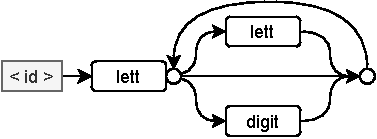
\includegraphics[scale = 1.3]{img/st.pdf}
  \caption{Esempio di carta sintattica in C, per un identificatore. Si legge
    ``un identificatore C 
    \textit{id} comincia sempre con una lettera alfabetica \textit{lett},
    seguita da una lettera alfabetica \textit{lett} o da una cifra
    \textit{digit}, il tutto iterato''. A esempio \texttt{A10} è un
    identificatore, \texttt{1AB} no.} 
  \label{fig:st}
\end{figure}
Quindi dal punto di vista della carta sintattica un'espressione è:
\begin{itemize}
  \item una costante
  \item una variabile
  \item un simbolo di funzione applicato a $n$ espressioni se il simbolo di
  funzione ha arietà $n$
\end{itemize}
Torniamo a parlare di logica predicativa.
\begin{definizione}
  Definiamo \textbf{termine chiuso} come un termine che non contiene variabili.
\end{definizione}
\begin{esempio}
  Ad esempio:
  \begin{itemize}
    \item $f(x,1)$, con $f$ di arietà 2, è un termine ma non è un termine
    chiuso, avendo $x$, che è una variabile, come argomento
    \item $g(4,7)$, con $g$ di arietà 2, è un termine ed è un termine chiuso,
    avendo solo costanti come argomento
    \item $g(f(x,2),4)$, con $g$ ed $f$ di arietà 2, è un termine, avendo una
    funzione ed una costante come parametri ed entrambi sono termini. Non è però
    un termine chiuso dato che $f(x,2)$ non è un termine chiuso
  \end{itemize}
\end{esempio}
\begin{definizione}
  Definiamo le \textbf{formule ben formate} del primo ordine. Si ha che:
  \begin{enumerate}
    \item se $P$ è un \textbf{predicato}, di arietà $n$ (cosa che potremmo
    indicare con $P^n$) e
    $t_1,\ldots, t_n$ sono \textbf{termini}, allora $P(t_1,\ldots, t_n)\in
    FBF$. $P(t_1,\ldots, t_n)$ è detta \textbf{formula atomica}
    \item se $\mathcal{A},\mathcal{B}\in FBF$ allora:
    \begin{itemize}
      \item $\neg \mathcal{A}\in FBF$
      \item $\mathcal{A}\land \mathcal{B}\in FBF$
      \item $\mathcal{A}\lor \mathcal{B}\in FBF$
      \item $\mathcal{A}\to \mathcal{B}\in FBF$
    \end{itemize}
    Si noti che $\mathcal{A}$ e $\mathcal{B}$, scritte così in corsivo per
    evidenziare questo aspetto, non fanno parte del linguaggio
    appena definito, non sono termini etc$\ldots$ ma sono \textbf{meta-variabili
      che variano su formule ben formate}, ovvero sono simboli di arbitrarie
    formule ben formate
    \item se $x$ è una \textbf{variabile individuale} e $P$ è un
    \textbf{predicato} del linguaggio, allora: 
    \begin{itemize}
      \item $\forall xP(x)\in FBF$
      \item $\exists xP(x)\in FBF$
    \end{itemize}
    Quindi i due quantificatori possono quantificare solo su variabili
    individuali (a livello di logica predicativa, ovvero di logica del primo
    ordine, una cosa del tipo $\forall P(P(x))$ non è ammessa)
  \end{enumerate}
\end{definizione}
Fin qui si potrebbe dire ``nulla di nuovo'', in quanto tutto quello che è appena
stato detto vale in logica intuizionistica come in logica classica. In realtà
qualche differenza potrei già farla. A livello di logica classica proposizionale
potrei usare un insieme minimale di operatori con solo $\neg$ e $\lor$ mentre in
logica intuizionistica non potrei. \\
Dal punto di vista dei quantificatori in
logica classica potrei definire $\forall$ come $\neg\exists\neg$ e $\exists$
come $\neg\forall\neg$, quindi me ne basterebbe uno dei due. In logica
intuizionistica questo non vale e i due quantificatori sono del tutto
indipendenti e non definibili, non valendo l'equivalenza classica.\\
Tra le due logiche quindi non si ha una differenza sintattica (al più che in
logica classica potrei togliere qualche connettore e un quantificatore) ma si ha
una differenza semantica (che spiega perché in logica intuizionistica non posso
trascurare connettivi e quantificatori).\\
Si avranno \textbf{modelli di Kripke} per la logica predicativa intuizionistica.
\begin{definizione}
  Si definisce \textbf{variabile libera} una variabile non legata ad un
  quantificatore. 
\end{definizione}
\begin{definizione}
  Definiamo \textbf{formula ben formata chiusa} quando ogni variabile della FBF
  compare nell'ambito di un quantificatore o esistenziale o universale. In altri
  termini una FBF è chiusa se non contiene variabili libere.\\
  Una FBF non chiusa si dice anche \textbf{FBF aperta}.
\end{definizione}
\begin{esempio}
  Ad esempio:
  \begin{itemize}
    \item $\forall x\exists yP(x,y)$ è una FBF chiusa
    \item $\forall x(P(x, y)\land Q(x))$ è una FBF ma non è una FBF chiusa a
    causa di $y$ 
    \item $\forall x(Q(x)\land \exists y(P(x,y)))$ è una FBF chiusa
     \item $\forall xQ(x)\land \exists y(P(x,y))$ è una FBF ma non è una FBF
     chiusa perché la $x$ del secondo termine dell'and non ha più un
     quantificatore (bisogna guardare le parentesi)
  \end{itemize}
\end{esempio}
\textit{Tendenzialmente studieremo formule ben formate chiuse} (in quanto
vedremo che ogni FBF chiusa è $\top$ e $\bot$ fissata un'interpretazione, che
dobbiamo ancora definire per la logica intuizionistica, mentre
una FBF aperta, per essere valutata, richiede una esemplificazione /
un'istanziazione della \textit{variabile libera}).
\subsection{Deduzione Naturale Predicativa}
Passiamo ora alla deduzione naturale in ottica logica predicativa.\\
Vediamo quindi l'estensione delle regole della deduzione naturale al caso
predicativo. A livello predicativo in realtà le regole sono le stesse della
logica classica in quanto basta la regola dell'eliminazione del $\neg$ a livello
proposizionale per caratterizzare anche la logica intuizionistica predicativa.\\
Anche in questo caso si hanno le regole di eliminazione e le regole di
introduzione, dato un predicato $P$ e $a$ costante:
\begin{table}[H]
  \Large
  \centering
  \begin{tabular}{c|c|c}
    quantificatore & introduzione & eliminazione\\
    \hline
    $\exists$ & $\frac{P(a)}{\exists xP(x)}i\exists$
                                  &$\frac{\stackrel{\pi}{\exists xP(x}),
                                    \stackrel{
                                    \stackrel{\cancel{P(a)}}{\pi_1}}{C}}{C}
                                    e\exists$\\
    \hline
    $\forall$ & $\frac{\stackrel{\pi}{P(x)}}{\forall xP(x)}i\forall$
                                  &$\frac{\forall xP(x)}{P(a)}e\forall$\\
  \end{tabular}
\end{table}
Per l'introduzione di $\forall$ non faccio ipotesi sul valore della costante $a$
e se ho una dimostrazione che porta a $P(a)$, dove non faccio appunto ipotesi su
$a$, allora posso introdurre il $\forall$. Mi serve quindi una dimostrazione di
$P(a)$ con $a$ non fissato. Si ha che $a$ in questo caso è quindi una sorta di
\textit{parametro} (questo vale anche nell'eliminazione del $\forall$, mentre
nell'introduzione di $\exists$ è una costante specifica, in quanto basta averne
una). Ad esempio posso dire che d ``pari 4'' posso dedurre che ``esiste un x
che è pari'' ma non che ``tutti gli x sono pari'', in quanto l'$a$
dell'introduzione del $\forall$ non deve essere specificato ma deve provenire da
una dimostrazione di $P(a)$ in cui $a $ non è mai stato particolarizzato.\\  
In merito all'eliminazione di $\exists$ si suppone di aver ottenuto $\exists
xP(x)$ tramite una dimostrazione $\pi$. Si assume quindi $P(x)$ dove $a$ non
deve essere mai occorso in nessun punto di $\pi$ e non dove occorrere in nessun
punto di $C$ che si ottiene tramite $\pi_1$. In tal caso posso eliminare
$\exists$ e ottenere $C$, che è indipendente dal valore di $a$ in $P(a)$. Ad
esempio posso dire ``esiste un numero primo e pari'', assumo un $Pari(a)$, e
deduco un $C$ che non contiene $a$, ad esempio $C=2$, allora posso eliminare
$\exists$ e concludere con 2 come risultante. Il punto è che a priori, da un
esiste, non so quale sia il termine esistente ma se faccio tutto il ragionamento
sopra posso dire che $C$ è tale termine e andare avanti nella dimostrazione.\\
Le \textit{regole critiche} sono l'introduzione di $\forall$, che è pesante come
significato dovendo dire che vale per ogni, e l'eliminazione dell'esiste, che è
pesante come significato in quanto dal dire che esiste qualcosa si estrae quel
qualcosa, arrivando ad un $C\in FBF$. Le altre due regole sono più
``leggere''.\\
Con queste quattro regole si ha un \textbf{calcolo corretto e completo} per la
logica classica se si ha l'eliminazione del $\neg$ e per la logica
intuizionistica se non si ha tale regola. Quindi questo calcolo, che ricordiamo
essere di Prawitz è molto flessibile e modulare rispetto alle varie logiche.\\
Tutte le altre regole proposizionali si usano come già visto.\\
La nozione di dimostrazione in deduzione naturale è invariata. Se scrivo
$\vdash_{INT}A$ intendo dire che è dimostrabile una formula predicativa $A$ in
logica intuizionistica, esistendo una sequenza finita di applicazioni di regole
di deduzione naturale predicativa intuizionistica che termina con la formula
$A$. Se ho assunzioni che non voglio scaricare posso dare la nozione più
generale di dimostrazione di una formula predicativa $A$ a partire da un insieme
di assunzioni $\Gamma$:
\[\Gamma\vdash_{INT} A\]
Vediamo qualche esempio di deduzione naturale predicativa.
\begin{esempio}
  Partiamo con un esempio famoso, di una formula non dimostrabile, nemmeno
  classicamente. Questo esempio segnala come l'uso scorretto dell'introduzione
  del $\forall$ può portare a dimostrazioni errate. Prendiamo quindi:
  \[\forall x(A(x)\lor B(x))\to\forall xA(x)\lor\forall xB(x)\]
  Ovvero avrei la ``distribuzione'' del $\forall$ sull'or che non ha
  senso. Sarebbe come dire ``ogni numero è pari o dispari quindi o ogni numero è
  pari o ogni numero è dispari''.\\
  Applichiamo le regole per vedere se è dimostrabile, sapendo che non dovrà
  esserlo.\\
  Si hanno le seguenti assunzioni:
  \begin{enumerate}
    \item $\forall x(A(x)\lor B(x))$
    \item $A(a)$
    \item $B(a)$
  \end{enumerate}
  E la dimostrazione:
  \begin{gather*}
    \frac{^1\forall x(A(x)\lor B(x))}{A(a)\lor B(a)}e\forall\\
    \mbox{In parallelo vorrei avere:}\\
    \frac{^2A(a)}{}i\forall,\,\,\frac{^3B(a)}{}i\forall\\
    \frac{\forall xA(x)}{}i\lor,\,\,\frac{\forall xB(x)}{}i\lor\\
    \frac{\forall xA(x)\lor\forall xB(x)}{},\,\,\frac{\forall xA(x)\lor\forall
      xB(x)}{} \\
    \mbox{Unendo i due percorsi:}\\
    \frac{A(a)\lor B(a), \forall xA(x)\lor\forall xB(x), \forall
      xA(x)\lor\forall xB(x)}{} \\
    \forall xA(x)\lor\forall xB(x)
  \end{gather*}
  \textbf{Non chiaro ipotetico ultimo passaggio, a priori del passaggio
    ``illegale''}.\\ 
  Ma questo non posso farlo perché per l'introduzione di $\forall$ non posso
  partire da assunzioni. Quindi questa formula non è nemmeno dimostrabile
  classicamente, come è intuitivo dire. Quindi:
  \[\nvdash_{CL}\forall x(A(x)\lor B(x))\to\forall xA(x)\lor\forall xB(x)\]
  Potenzialmente potrei avere altri metodi ma possiamo dire che, in questo caso,
  non si arriverebbe mai a conclusione.
\end{esempio}
\textit{Si può dimostrare che l'$\exists$ si distribuisce sull'or (fatto su
  quaderno)}.\\ 
Vediamo ora un altro esempio.
\begin{esempio}
  Vediamo un esempio di formula dimostrabile solo classicamente:
  \[\exists xA(x)\iff \neg \forall x\neg A(x)\]
  Vedremo che uno dei due sensi è dimostrabile anche intuizionisticamente.\\
  Parto con:
  \[\exists xA(x)\to \neg \forall x\neg A(x)\]
  Si hanno le assunzioni:
  \begin{enumerate}
    \item $\exists xA(x)$
    \item $\forall x\neg A(x)$
    \item $A(a)$
  \end{enumerate}
  e la seguente applicazione di regole:
  \begin{gather*}
    \frac{^2\cancel{\forall x\neg A(x)}}{}e\forall\\
    \frac{^3 \cancel{A(a)}, \neg A(a)}{}i\bot\\
    \frac{\bot}{}i\neg\mbox{(scaricando 2)}\\
    \frac{^1\cancel{\exists xA(x)},\neg\forall x\neg
      A(x)}{}e\exists\mbox{(scaricando 3)}\\
    \frac{\neg\forall x\neg A(x)}{}i\to\mbox{(scaricando 1)}\\
    \exists x A(x)\to  \neg \forall x\neg A(x)
  \end{gather*}
  Quindi la formula è dimostrabile intuizionisticamente, non avendo assunzioni
  non scaricate. \textit{Come strategia si è seguita quella simile alla logica
  proposizionale, cercando di arrivare all'introduzione finale dell'implica che
  scaricasse la prima assunzione}.\\
  Vedo l'altro verso:
  \[\exists xA(x)\gets \neg \forall x\neg A(x)\]
  ovvero:
  \[\neg \forall x\neg A(x)\to\exists xA(x)\]
  \emph{Si ragiona sapendo che la dimostrazione è possibile solo
    classicamente}.\\
  Si hanno le assunzioni:
  \begin{enumerate}
    \item $\neg \forall\neg x A(x)$
    \item $\neg A(a)$
  \end{enumerate}
  e la seguente applicazione di regole:
  \begin{gather*}
    \frac{^2\cancel{\neg A(a)}}{}i\forall\\
    \frac{^1 \neg \forall\neg x A(x),\forall x \neg A(x)}{}i\bot\\
    \frac{\bot}{}e\neg\mbox{(scaricando 2)}\\
    \frac{A(a)}{}i\exists\\
    \frac{\exists xA(x)}{}i\to\mbox{(scaricando 1)}\\
    \neg \forall x\neg A(x)\to\exists xA(x)
  \end{gather*}
  L'introduzione del $\neg$ è solo presente in logica classica e non in logica
  intuizionistica.\\
  \textbf{Come prima si potrebbe pensare che non va bene perché introduco il
    $\forall$ da un'assunzione, ma l'assunzione poi viene scaricata, siamo
    quindi ``al limite'' dell'accettabile}.\\ 
  Si ha comunque che la formula è dimostrabile solo classicamente per
  l'introduzione del $\neg$.\\
  Cerchiamo ora un'altra dimostrazione senza quell'introduzione di $\forall$
  ``al limite'' (anche se la dimostrazione sopra sarebbe accettata in esame).\\
  Si hanno le assunzioni:
  \begin{enumerate}
    \item $\neg \forall\neg x A(x)$
    \item $\neg \exists xA(x)$
  \end{enumerate}
  Si usa il lemma per cui da $\neg \exists xA(x)$ derivo $\forall x\neg A(x)$.\\
  Si ha quindi la seguente applicazione di regole:
  \begin{gather*}
    \frac{^2\cancel{\neg \exists xA(x)}}{\rule{49pt}{0.4pt}}\mbox{(regola
      derivata)}\\ 
    \\
    \frac{^1\cancel{\neg \forall\neg x A(x)}, \forall x\neg A(x)}{}i\bot\\
    \frac{\bot}{}i\neg\mbox{(scaricando 2)}\\
    \frac{\exists x A(x)}{}i\to\mbox{(scaricando 1)}\\
    \neg \forall x\neg A(x)\to\exists xA(x)
  \end{gather*}
  Si ha comunque che la formula è dimostrabile solo classicamente e non
  intuizionisticamente, per 
  l'introduzione del $\neg$, al più comunque di riuscire dimostrare,
  classicamente il lemma:
  \[\vdash_{CL}\neg\exists x A(x)\to \forall x \neg A(x)\]
  Vediamo tale dimostrazione.\\
  Si assume:
  \begin{enumerate}
    \item $A(a)$
    \item $\neg \exists A(x)$
  \end{enumerate}
  Avendo quindi la seguente applicazione di regole:
  \begin{gather*}
    \frac{^1\cancel{A(a)}}{}i\exists\\
    \frac{^2\cancel{\neg \exists A(x)},\exists x A(x)}{}i\bot\\
    \frac{\bot}{}i\neg\mbox{(scaricando 1)}\\
    \frac{\neg A(a)}{}i\forall\\
    \frac{\forall x\neg A(x)}{}i\to\mbox{(scaricando 2)}\\
    \neg\exists x A(x)\to \forall x \neg A(x)
  \end{gather*}
  Avendo che la formula è dimostrabile classicamente.\\
  \textbf{Posso fare l'introduzione di $\forall$ perché $\neg A(a)$ è
    derivata e $a$ compare solo in una formula derivata.}\\
  Del resto quest'ultima  dimostrazione
  sarebbe valida anche intuizionisticamente se ci servisse. Quindi si ha che:
  \[\vdash_{INT}\neg\exists x A(x)\to \forall x \neg A(x)\] 
\end{esempio}
\textit{Chiamo il seguente teorema anche se non ho idea di cosa sia
  veramente.}\\ 
\begin{teorema}
  Nell'intuizionismo non è mai dimostrabile che da una formula negata si arrivi
  ad un esistenziale ``puro''. 
\end{teorema}
\end{document}

% LocalWords:  clock  Bayesana machine learning Bayes riscalare Prolog Morgan
% LocalWords:  condizionalmente l'algoritmicità tableaux intuizionisticamente
% LocalWords:  l'istanziazione Kripke contromodello sottoformule Kolmogorov sse
% LocalWords:  Glivenko incorporariamo sequenti  implicazionale implicazionali
% LocalWords:  branch arietà un'istanziazione
